% =============================================================================
% MASTER'S THESIS — Institute of Science and Technology, Tribhuvan University
% Title: Enhancing Self-Supervised Video Representations with HAF-STD Net: A Comparative Evaluation Against VLM for Action Recognition
% Standard: IoST TU Research Regulation 2025 & APA 7th Edition Reference Style
% =============================================================================

\documentclass[a4paper, 12pt]{report}

% --- Geometry & Spacing ------------------------------------------------------
\usepackage[top=1in, bottom=1in, left=1.5in, right=1in]{geometry}
\usepackage{times}                    % Times New Roman font
\usepackage{setspace}                 % 1.5 line spacing
\onehalfspacing
\usepackage{microtype}                % Subtle font expansion/protrusion for better line breaks

% --- Hyphenation & Overflow Control ------------------------------------------
\hyphenpenalty=10000                  % Effectively disable mid-word hyphenation
\exhyphenpenalty=10000                % Effectively disable breaks at explicit hyphens
\tolerance=9999                      % Allow very loose spacing to avoid hyphenation
\emergencystretch=3em                % Extra stretch to prevent words overflowing margins

% --- Packages ----------------------------------------------------------------
\usepackage{graphicx}
\usepackage{amsmath, amssymb}
\usepackage{booktabs}
\usepackage{longtable}
\usepackage{multirow}
\usepackage{array}
\usepackage{tabularx}
\usepackage{float}
\usepackage{caption}
\usepackage{subcaption}
\usepackage[hidelinks]{hyperref}
\usepackage{url}
\usepackage{pdfpages}                 % Include external PDF pages (Nepali abstract)
\usepackage[style=apa, backend=biber, natbib=true]{biblatex}
\addbibresource{references.bib}
\usepackage{algorithm}
\usepackage{algorithmic}
\usepackage{listings}
\usepackage{xcolor}
\usepackage{tikz}
\usepackage{pgfplots}
\pgfplotsset{compat=1.18}
\usetikzlibrary{shapes,arrows,positioning,calc}
\usepackage{enumitem}
\usepackage{fancyhdr}
\usepackage{tocloft}
\usepackage{titlesec}

% --- Custom Colors & Environments for Code Explanations ---------------------
\definecolor{codebg}{RGB}{248,248,248}
\definecolor{codegreen}{RGB}{0,128,0}
\definecolor{codepurple}{RGB}{128,0,128}
\definecolor{codegray}{RGB}{100,100,100}
\definecolor{codeblue}{RGB}{0,0,180}
\definecolor{codeorange}{RGB}{200,80,0}

\newenvironment{explanation}{%
  \par\smallskip
  \noindent\textcolor{blue!70!black}{\textbf{Explanation:}}\\
  \noindent
}{\par\medskip}

% --- biblatex-apa provides \citep, \citet, \citealp natively via natbib=true --

% --- Heading Sizes (as per IoST regulation) ----------------------------------
\titleformat{\chapter}[display]
  {\normalfont\fontsize{16}{20}\bfseries\centering}
  {\chaptertitlename\ \thechapter}{10pt}{\fontsize{16}{20}\bfseries\centering}
\titleformat{\section}
  {\normalfont\fontsize{14}{18}\bfseries}{\thesection}{1em}{}
\titleformat{\subsection}
  {\normalfont\fontsize{12}{15}\bfseries}{\thesubsection}{1em}{}
\titleformat{\subsubsection}
  {\normalfont\fontsize{12}{15}\bfseries}{\thesubsubsection}{1em}{}

% --- Page style --------------------------------------------------------------
\pagestyle{fancy}
\fancyhf{}
\fancyfoot[C]{\thepage}
\renewcommand{\headrulewidth}{0pt}

% --- Caption style (IoST Regulation 10.7 & Appendix K/L: Only No. in Bold, Justified) -
\captionsetup{font=normalsize, labelfont=bf, textfont=normalfont, labelsep=colon, justification=justified, singlelinecheck=true}
\captionsetup[table]{position=above}
\captionsetup[figure]{position=below}

% --- Continuous Sequential Numbering (IoST Regulation 10.7 d, 10.8) ----------
\counterwithout{figure}{chapter}
\counterwithout{table}{chapter}
\numberwithin{equation}{chapter}                 % Equation numbering by chapter: 3.1, 3.2, ...

% --- Photo Plate Float Environment (IoST Regulation 10.7) --------------------
\newfloat{photoplate}{htbp}{lop}
\floatname{photoplate}{Photo plate}
\counterwithout{photoplate}{chapter}
\newcommand{\listofphotoplates}{\listof{photoplate}{List of Photo Plates}}

% --- List of Tables & Figures Formatting (IoST Regulation Appendix K & L) -----
\renewcommand{\cfttabpresnum}{\bfseries Table }
\renewcommand{\cfttabaftersnum}{\textbf{:}\normalfont}
\settowidth{\cfttabnumwidth}{\textbf{Table 99: }}
\setlength{\cfttabindent}{0pt}

\renewcommand{\cftfigpresnum}{\bfseries Figure }
\renewcommand{\cftfigaftersnum}{\textbf{:}\normalfont}
\settowidth{\cftfignumwidth}{\textbf{Figure 99: }}
\setlength{\cftfigindent}{0pt}


% --- Code listing style ------------------------------------------------------
\lstset{
  language=Python,
  backgroundcolor=\color{codebg},
  basicstyle=\scriptsize\ttfamily,
  breaklines=true,
  breakatwhitespace=false,
  breakautoindent=true,
  breakindent=1.5em,
  columns=flexible,
  numbers=left,
  numberstyle=\tiny\color{codegray},
  keywordstyle=\color{codeblue}\bfseries,
  commentstyle=\color{codegreen}\itshape,
  stringstyle=\color{codeorange},
  tabsize=2,
  showstringspaces=false,
  xleftmargin=1.5em,
  xrightmargin=0.5em,
}

% --- Author & Thesis Variables -----------------------------------------------
\newcommand{\studentname}{Erize Rai}
\newcommand{\authorname}{\studentname}
\newcommand{\studentroll}{8025006}
\newcommand{\studentregno}{5-3-28-193-2023}
\newcommand{\supervisorname}{Asst. Prof. Dr. Dhiraj Kedar Pandey}
\newcommand{\supervisordesignation}{Assistant Professor}
\newcommand{\cosupervisorname}{}
\newcommand{\cosupervisordesignation}{}
\newcommand{\externalexaminer}{Asst. Prof. Surya Bahadur Bam}
\newcommand{\externaldesignation}{Bhaktapur Multiple Campus}
\newcommand{\internalexaminer}{Asst. Prof. Dr. Arjun Saud}
\newcommand{\internaldesignation}{Assistant Professor}
\newcommand{\hodname}{Asst. Prof. Dr. Dhiraj Kedar Pandey}
\newcommand{\thesistitle}{Enhancing Self-Supervised Video Representations with HAF-STD Net: A Comparative Evaluation Against VLM for Action Recognition}
\newcommand{\submissionmonthyear}{NOVEMBER, 2026}
\newcommand{\submissiondate}{NOVEMBER, 2026}

% --- Custom commands ---------------------------------------------------------
\newcommand{\vjepaa}{V-JEPA~2.1}
\newcommand{\qwenvl}{Qwen2.5-VL}

% =============================================================================
\begin{document}

% Roman numerals for front matter
\pagenumbering{roman}

% --- Front Matter (IoST Section 10.1 order) ----------------------------------
% =============================================================================
%        FORMAT OF TITLE AND COVER PAGES SAMPLE OF THESIS (Appendix B)
% =============================================================================

\begin{titlepage}
\centering

{\fontsize{18}{22}\selectfont \textbf{\thesistitle}}\\[1.2cm]

% Logo of T.U.: Center, size 2" x 2"

\includegraphics[width=2in, height=2in, keepaspectratio]{fig/tulogo.png}\\[1.2cm]

% Partial fulfillment text: Times New Roman, Capitalize each word, Bold, Center aligned, Font size 14
{\fontsize{14}{18}\selectfont \textbf{A Thesis Submitted for the Partial Fulfillment of the Requirements for}}\\
{\fontsize{14}{18}\selectfont \textbf{the Master's in Information Technology}}\\[0.8cm]

% Submitted to: Times New Roman, Capitalize each word, Bold, Center aligned, Font size 14
{\fontsize{14}{18}\selectfont \textbf{Submitted to the}}\\
{\fontsize{14}{18}\selectfont \textbf{Central Department of Computer Science and Information Technology}}\\
{\fontsize{14}{18}\selectfont \textbf{Institute of Science and Technology}}\\
{\fontsize{14}{18}\selectfont \textbf{Tribhuvan University}}\\
{\fontsize{14}{18}\selectfont \textbf{NEPAL}}\\[0.8cm]

% "By": Center, Bold, Font size 14
{\fontsize{14}{18}\selectfont By}\\[0.4cm]

% Student details: Times New Roman, Capitalize each word, Bold, Center aligned, Font size 14
{\fontsize{14}{18}\selectfont \textbf{\studentname}}\\
{\fontsize{14}{18}\selectfont \textbf{Exam Roll No. \studentroll}}\\
{\fontsize{14}{18}\selectfont \textbf{T.U. Registration No. \studentregno}}\\[1.0cm]

% Month, YYYY: Times New Roman, Upper case, Bold, Center aligned, Font size 14
{\fontsize{14}{18}\selectfont \textbf{\submissionmonthyear}}

\end{titlepage}
          % i.    Cover Page / Inner Cover Page
% =============================================================================
%                   APPENDIX C: DECLARATION FROM THE STUDENT
% =============================================================================

\newpage
\phantomsection
\addcontentsline{toc}{chapter}{Declaration}

\begin{center}
{\fontsize{16}{20}\selectfont \textbf{Declaration}}
\end{center}

\vspace{0.5cm}

\noindent
This thesis entitled \textbf{``\thesistitle''} which is being submitted to the Central Department of Computer Science and Information Technology, Institute of Science and Technology (IoST), Tribhuvan University, Nepal for the partial fulfillment of the requirement to the Master of Science Degree in Information Technology has been carried out by me under the supervision of \textbf{\supervisorname} at Central Department of Computer Science and Information Technology. This work is original and has not been submitted earlier in part or full in this or any other form to any other institution for the award of any degree.

\vspace{3cm}

\noindent
\begin{tabular}{@{}l}
\rule{6cm}{0.4pt} \\
\textbf{\studentname} \\
\end{tabular}

\vspace{1cm}
\noindent
Date: \submissiondate
        % iv.   Declaration
% =============================================================================
%              APPENDIX D: RECOMMENDATION FROM THE SUPERVISOR
% =============================================================================

\newpage
\phantomsection
\addcontentsline{toc}{chapter}{Recommendation}

\begin{center}
{\fontsize{16}{20}\selectfont \textbf{Recommendation}}
\end{center}

\vspace{0.5cm}

\noindent
This is to recommend that {\studentname} has carried out the thesis entitled \textbf{``\thesistitle''} for the partial fulfillment of the requirement of Master's in Information Technology under my supervision. To the best of my knowledge, this work has not been submitted to any other institution for any academic degree. He has fulfilled all the requirements of the Central Department of Computer Science and Information Technology, Institute of Science and Technology (IoST), Tribhuvan University, Nepal for the submission of the thesis for the Master's degree in Information Technology.

\vspace{2.5cm}

\noindent
\begin{tabular}{@{}p{8.5cm}}
\rule{6cm}{0.4pt} \\
\textbf{Supervisor} \\
\supervisorname \\
\supervisordesignation \\
Central Department of Computer Science and \\
Information Technology \\
Tribhuvan University \\
Kathmandu, Nepal \\
\end{tabular}

\vspace{1.5cm}

\begin{center}
{\fontsize{12}{15}\selectfont \textbf{\submissiondate}}
\end{center}
     % v.    Recommendation
% =============================================================================
%                   APPENDIX E: LETTER OF APPROVAL
% =============================================================================

\newpage
\phantomsection
\addcontentsline{toc}{chapter}{Letter of Approval}

\begin{center}
{\fontsize{16}{20}\selectfont \textbf{Letter of Approval}}
\end{center}

\vspace{0.5cm}

\noindent
The thesis work entitled \textbf{``\thesistitle''} submitted at the Central Department of Computer Science and Information Technology, Institute of Science and Technology, Tribhuvan University by {\studentname} has been accepted for the partial fulfillment of Master's in Information Technology.

\vspace{2.0cm}

\noindent
\begin{tabular}{@{}p{7.5cm}p{7.5cm}@{}}
\rule{6cm}{0.4pt} & \rule{6cm}{0.4pt} \\
\textbf{External Examiner} & \textbf{Internal Examiner} \\[0.2cm]
\begin{tabular}[t]{@{}l@{}}
Asst. Prof. Surya Bahadur Bam \\
Bhaktapur Multiple Campus \\
Tribhuvan University \\
Bhaktapur, Nepal
\end{tabular}
&
\begin{tabular}[t]{@{}l@{}}
Asst. Prof. Dr. Arjun Saud \\
Central Department of Computer Science \\
and Information Technology \\
Tribhuvan University \\
Kathmandu, Nepal
\end{tabular}
\end{tabular}

\vspace{2.2cm}

\noindent
\begin{tabular}{@{}p{7.5cm}p{7.5cm}@{}}
\rule{6cm}{0.4pt} & \rule{6cm}{0.4pt} \\
\textbf{Supervisor} & \textbf{Head of the Department} \\[0.2cm]
\begin{tabular}[t]{@{}l@{}}
\supervisorname \\
Central Department of Computer Science \\
and Information Technology \\
Tribhuvan University \\
Kathmandu, Nepal
\end{tabular}
&
\begin{tabular}[t]{@{}l@{}}
\hodname \\
Central Department of Computer Science \\
and Information Technology \\
Tribhuvan University \\
Kathmandu, Nepal
\end{tabular}
\end{tabular}

\vspace{1cm}

\begin{center}
{\fontsize{12}{15}\selectfont \textbf{\submissionmonthyear}}
\end{center}

           % vi.   Letter of Approval
% =============================================================================
%                     APPENDIX F: ACKNOWLEDGEMENTS
% =============================================================================

\newpage
\phantomsection
\addcontentsline{toc}{chapter}{Acknowledgements}

\begin{center}
{\fontsize{16}{20}\selectfont \textbf{Acknowledgements}}
\end{center}

\vspace{0.5cm}

\noindent
First and foremost, I extend my deepest appreciation to my supervisor, \textbf{\supervisorname}, for their continuous guidance, motivation, and invaluable feedback throughout this research. Their insightful suggestions and constructive criticism provided during every stage of this work were instrumental in shaping the direction and quality of this thesis.

I am grateful to the Central Department of Computer Science and Information Technology, Institute of Science and Technology, Tribhuvan University, for providing the academic environment and resources necessary for this research. 

Finally, I express my heartfelt gratitude to my family and friends for their unwavering support, patience, and encouragement throughout my graduate studies.

\vspace{1.5cm}
\noindent
\begin{tabular}{@{}l}
\rule{6cm}{0.4pt} \\
{\studentname} \\
\submissionmonthyear \\
\end{tabular}
    % vii.  Acknowledgements
% % =============================================================================
%                    PLAGIARISM TEST REPORT
% =============================================================================
\chapter*{Plagiarism Test Report}
\addcontentsline{toc}{chapter}{Plagiarism Test Report}

\textit{}
         %       Plagiarism Test Report
% =============================================================================
%                         APPENDIX G: ABSTRACT
% =============================================================================

\newpage
\phantomsection
\addcontentsline{toc}{chapter}{Abstract}

\begin{center}
{\fontsize{16}{20}\selectfont \textbf{Abstract}}
\end{center}

\vspace{0.5cm}

\noindent
This thesis investigates the comparative effectiveness of self-supervised video encoder and vision-language model for video action recognition. Two state-of-the-art foundation models representing fundamentally different learning paradigms were evaluated: V-JEPA~2.1 (654M parameters), a self-supervised video encoder from Meta AI trained via masked spatio-temporal prediction in latent space, and Qwen2.5-VL (7B parameters), an autoregressive vision-language model from Alibaba Cloud. A frozen-feature evaluation protocol was employed on two complementary benchmarks: FineGym (4-class fine-grained gymnastics classification, 1,200 clips) and HMDB51 (51-class coarse-grained action recognition, 6,754 videos). The extracted representations were evaluated across nine classifiers, including three classical machine learning algorithms, five neural network classifiers, and a novel HAF-STD Net (Hierarchical Adaptive Fusion with Spectral-Temporal Decomposition) architecture designed to exploit multi-layer latent representations. On FineGym, V-JEPA~2.1 paired with HAF-STD Net achieved 98.1\% accuracy and 97.8\% macro F1, outperforming Qwen2.5-VL's best result (89.1\% accuracy, 88.4\% macro F1 with DeepMLP) by a 9.4 percentage point F1 margin. On HMDB51, V-JEPA~2.1 with HAF-STD Net achieved 84.7\% accuracy and 85.3\% macro F1, surpassing Qwen2.5-VL's best result (77.1\% accuracy, 79.1\% macro F1 with DeepMLP) by a 6.2 percentage point F1 margin. The results demonstrate that task-specialized self-supervised video encoders produce substantially more discriminative temporal representations than general-purpose VLMs, despite operating with an order of magnitude fewer parameters. Furthermore, the proposed HAF-STD Net shows that decomposing multi-layer latent representations into hierarchical appearance, motion, and depth-velocity streams through adaptive routing yields significant performance gains for frozen self-supervised video backbones.

\vspace{0.8cm}
\noindent
{\fontsize{10}{13}\selectfont \textit{Keywords: Video Understanding, Self-Supervised Learning, Vision-Language Models, V-JEPA 2.1, Qwen2.5-VL, Action Recognition, HAF-STD Net}}

           % viii. Abstract
% =============================================================================
%                    शोधसार (ABSTRACT IN NEPALI)
% =============================================================================
% IoST Research Regulation 2025, Appendix H
%
% This page includes a pre-compiled PDF (via XeLaTeX with Mangal font).
% To regenerate:
%   cd frontmatter
%   xelatex abstract_nepali_standalone.tex
%
% Requires \usepackage{pdfpages} in the main preamble.
% =============================================================================

\newpage
\phantomsection
\addcontentsline{toc}{chapter}{\protect\raisebox{-0.15ex}{\protect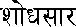
\includegraphics[height=1.05em]{frontmatter/shodhasaar_label.pdf}}}
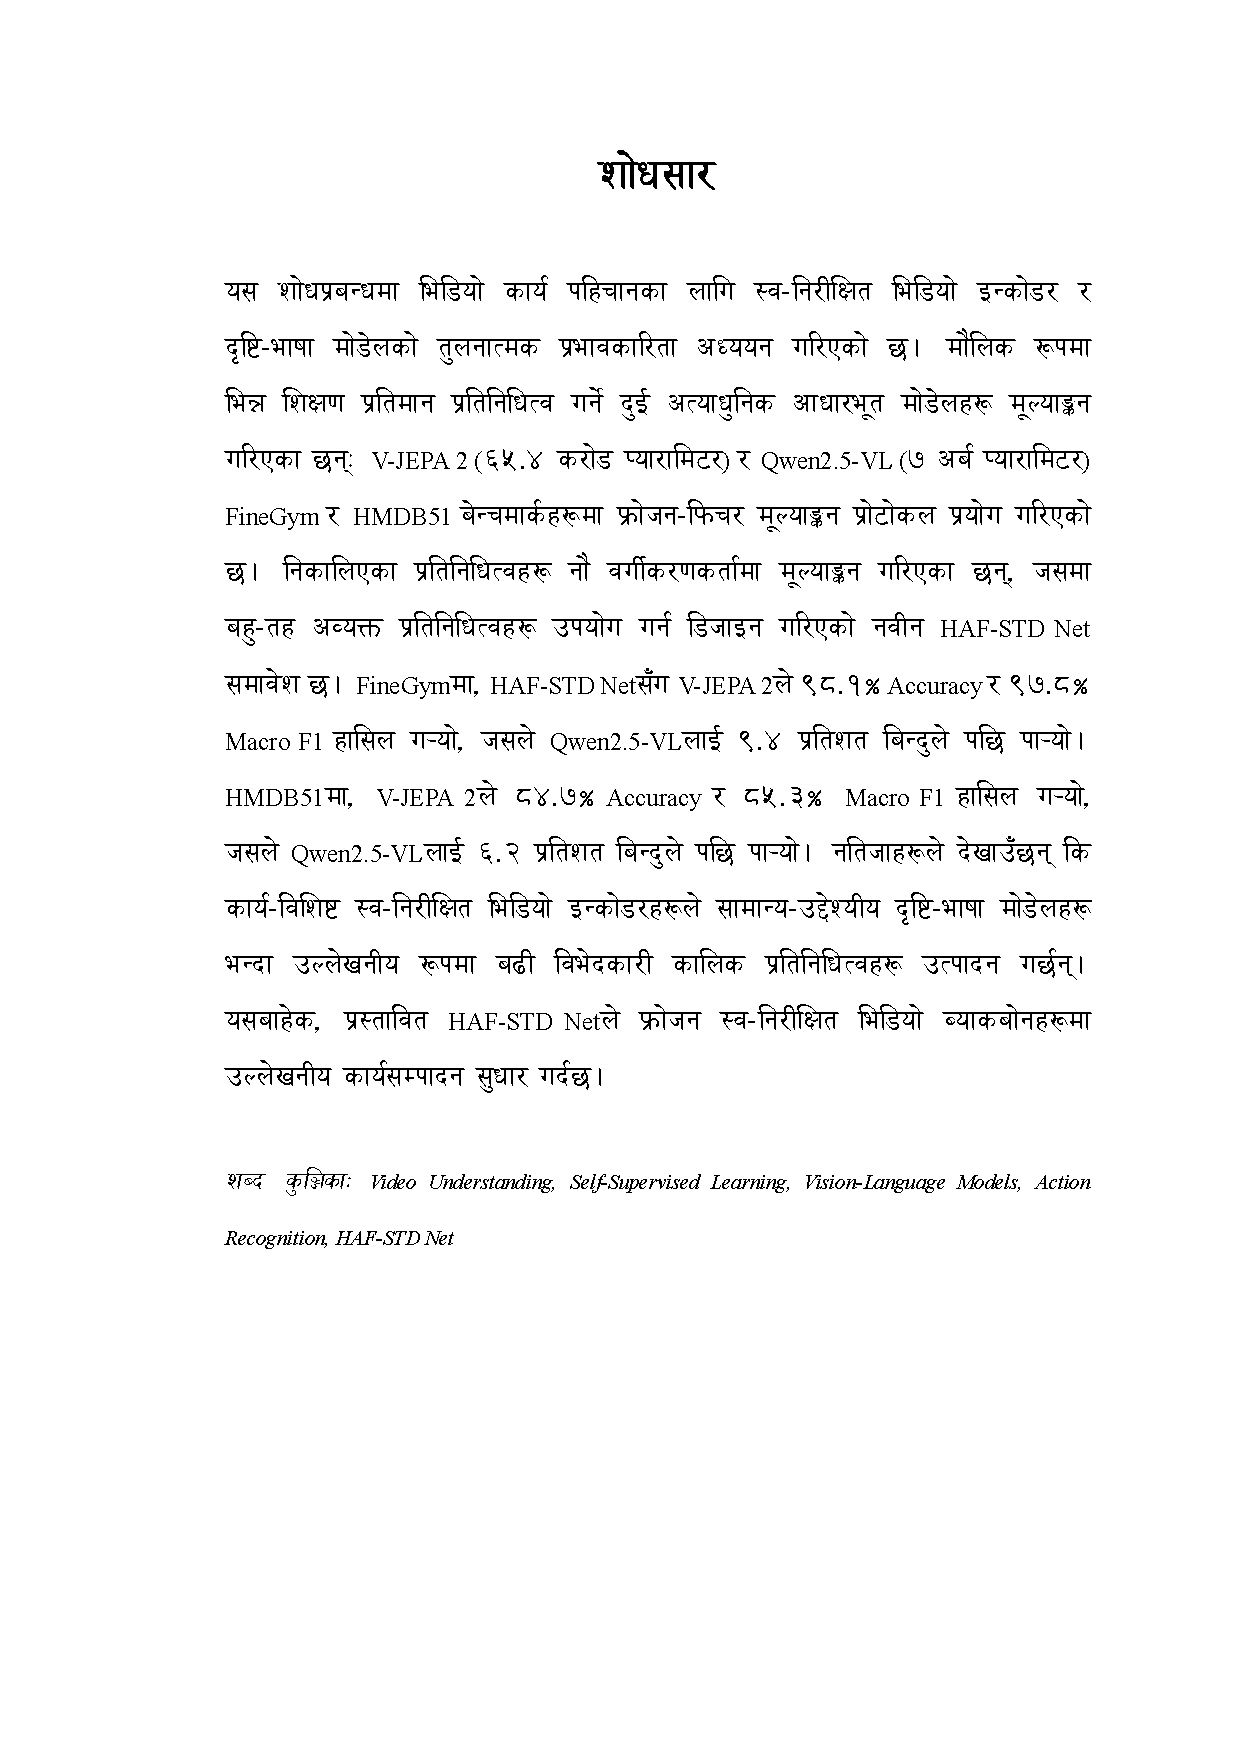
\includepdf[pages=-,pagecommand={\thispagestyle{fancy}}]{frontmatter/abstract_nepali_standalone.pdf}
    % ix.   शोधसार (Abstract in Nepali)

% =============================================================================
%        APPENDIX I: LIST OF ABBREVIATIONS AND ACRONYMS
% =============================================================================

\newpage
\phantomsection
\addcontentsline{toc}{chapter}{List of Abbreviations and Acronyms}

\begin{center}
{\fontsize{16}{20}\selectfont \textbf{List of Abbreviations and Acronyms}}
\end{center}

\vspace{0.5cm}

\begin{longtable}{@{}p{3.5cm}p{10.5cm}@{}}
\toprule
\textbf{Abbreviation} & \textbf{Full Form} \\
\midrule
\endhead
AdamW & Adam with Decoupled Weight Decay \\
AI & Artificial Intelligence \\
BB & Balance Beam \\
BERT & Bidirectional Encoder Representations from Transformers \\
BnB & BitsAndBytes (Quantization Library) \\
C3D & 3D Convolutional Network \\
CLIP & Contrastive Language-Image Pre-Training \\
CNN & Convolutional Neural Network \\
CUDA & Compute Unified Device Architecture \\
DWT & Discrete Wavelet Transform \\
EMA & Exponential Moving Average \\
FPS & Frames Per Second \\
FX & Floor Exercise \\
GELU & Gaussian Error Linear Unit \\
GFLOPs & Giga Floating Point Operations Per Second \\
GPU & Graphics Processing Unit \\
HAF-STD & Hierarchical Adaptive Fusion with Spectral-Temporal Decomposition \\
HMDB & Human Motion DataBase \\
HOF & Histogram of Optical Flow \\
HOG & Histogram of Oriented Gradients \\
I3D & Inflated 3D Convolutional Network \\
iDT & Improved Dense Trajectories \\
IoST & Institute of Science and Technology \\
JEPA & Joint Embedding Predictive Architecture \\
LLM & Large Language Model \\
LM & Language Model \\
LSTM & Long Short-Term Memory \\
MAE & Masked Autoencoder \\
MCC & Matthews Correlation Coefficient \\
MIT & Master of Information Technology \\
MLP & Multi-Layer Perceptron \\
MRoPE & Multimodal Rotary Position Embedding \\
MViT & Multiscale Vision Transformer \\
NF4 & Normal Float 4-bit (Quantization Format) \\
NLP & Natural Language Processing \\
OOM & Out of Memory \\
PCA & Principal Component Analysis \\
RBF & Radial Basis Function \\
ReLU & Rectified Linear Unit \\
RNN & Recurrent Neural Network \\
RoPE & Rotary Position Embedding \\
SDPA & Scaled Dot-Product Attention \\
SSL & Self-Supervised Learning \\
SVM & Support Vector Machine \\
TU & Tribhuvan University \\
UB & Uneven Bars \\
V-JEPA & Video Joint Embedding Predictive Architecture \\
VideoMAE & Video Masked Autoencoder \\
ViT & Vision Transformer \\
VLM & Vision-Language Model \\
VRAM & Video Random Access Memory \\
VT & Vault \\
\bottomrule
\end{longtable}
      % x.    List of Abbreviations and Acronyms

% =============================================================================
%                   APPENDIX J: LIST OF SYMBOLS
% =============================================================================

\newpage
\phantomsection
\addcontentsline{toc}{chapter}{List of Symbols}

\begin{center}
{\fontsize{16}{20}\selectfont \textbf{List of Symbols}}
\end{center}

\vspace{0.5cm}

\begin{longtable}{@{}p{3.5cm}p{10.5cm}@{}}
\toprule
\textbf{Symbol} & \textbf{Description} \\
\midrule
\endhead
$\mathbf{x}$ & Input Video Clip / Spatio-Temporal Frame Sequence \\
$\mathbf{z}$ & Latent Feature Representation Vector \\
$\mathbf{y}$ & Ground-Truth Action Class Label \\
$\hat{\mathbf{y}}$ & Predicted Action Class Label Probability Distribution \\
$\mathcal{L}_{\text{CE}}$ & Cross-Entropy Loss Function \\
$\mathcal{L}_{\text{Smooth}}$ & Label-Smoothing Cross-Entropy Loss Function \\
$\epsilon$ & Label-Smoothing Hyperparameter ($\epsilon = 0.1$) \\
$\alpha$ & Mixup Interpolation Beta Distribution Parameter ($\alpha = 0.2$) \\
$\lambda$ & Weight Decay / Regularization Parameter ($\lambda = 10^{-4}$) \\
$\eta$ & Learning Rate \\
$\kappa$ & Cohen's Kappa Coefficient \\
$\sigma(\cdot)$ & Softmax / Sigmoid Activation Function \\
$\mathbb{E}$ & Mathematical Expectation Operator \\
$d_{\text{embed}}$ & Embedding Dimension ($1280$ for V-JEPA 2, $3584$ for Qwen2.5-VL) \\
$N_{\text{frames}}$ & Number of Sampled Video Frames ($8$ for V-JEPA 2, $4$ for Qwen2.5-VL) \\
$C$ & Number of Target Action Classes ($4$ for FineGym, $51$ for HMDB51) \\
\bottomrule
\end{longtable}
            % xi.   List of Symbols

\newpage
\phantomsection
\addcontentsline{toc}{chapter}{List of Tables}
\begingroup
\renewcommand*{\addvspace}[1]{}
\listoftables                          % xii.  List of Tables
\endgroup

\newpage
\phantomsection
\addcontentsline{toc}{chapter}{List of Figures}
\begingroup
\renewcommand*{\addvspace}[1]{}
\listoffigures                         % xiii. List of Figures
\endgroup

\newpage
\phantomsection
\addcontentsline{toc}{chapter}{Table of Contents}
\tableofcontents                       % xiv.  Table of Contents

% =============================================================================
%      MAIN REPORT — Arabic numerals from here (Page 1)
% =============================================================================
\newpage
\pagenumbering{arabic}
\setcounter{page}{1}
\setcounter{table}{0}
\setcounter{figure}{0}

% --- 5 Main Chapters (IoST CS/IT Format) --------------------------------------
% =============================================================================
%               CHAPTER 1: INTRODUCTION
% =============================================================================
\chapter{Introduction}

\section{General Introduction and Background}

Video understanding represents one of the most challenging frontiers in computer vision and artificial intelligence research. Unlike static image recognition, which has seen remarkable progress over the past decade, video comprehension demands that models capture not only spatial features within individual frames but also the complex temporal dynamics that unfold across sequences of frames \citep{bardes2024vjepa}. This temporal dimension introduces an exponential increase in computational complexity and representational challenges, making video understanding a substantially more demanding task than its image-based counterpart.

Action recognition---the task of identifying human activities from video data---is a central problem in video understanding with broad applications spanning sports analytics, surveillance, human-computer interaction, healthcare monitoring, and content-based video retrieval \citep{bordes2024vlm}. The difficulty of action recognition varies dramatically depending on the granularity of the target classes: coarse-grained recognition of clearly distinct activities (e.g., ``running'' vs.\ ``swimming'') differs fundamentally from fine-grained recognition of visually similar activities (e.g., distinguishing between gymnastics events that occur in similar arenas).

Two fundamentally different paradigms have emerged for learning video representations in recent years. The first is self-supervised learning (SSL), where models learn representations from unlabeled video data by solving pretext tasks such as predicting masked regions in latent feature space \citep{assran2023ijepa, assran2025vjepa2, murlabadia2026vjepa21}. The second is vision-language modelling (VLM), where models are trained on large-scale paired image/video and text data using autoregressive language modelling objectives \citep{bordes2024vlm, bai2025qwen2vl}. Both paradigms have produced models that achieve impressive results on a wide range of benchmarks, yet their relative merits across different recognition granularities remain insufficiently explored.

The rise of foundation models has intensified this question: self-supervised video encoders such as V-JEPA~2.1 \citep{assran2025vjepa2, murlabadia2026vjepa21} are trained exclusively on visual data, learning representations through masked spatio-temporal prediction without any linguistic supervision. In contrast, vision-language models like Qwen2.5-VL \citep{bai2025qwen2vl} are trained on massive corpora of paired image-text and video-text data, acquiring both visual and semantic understanding through autoregressive generation. Whether the additional linguistic grounding in VLMs translates to better video representations for discriminative tasks---or whether it introduces noise that dilutes task-relevant temporal features---remains an open empirical question.

This thesis addresses this gap by presenting a systematic comparative analysis of a leading model from each paradigm: V-JEPA~2.1 \citep{assran2025vjepa2, murlabadia2026vjepa21}, a self-supervised video encoder developed by Meta AI with 654 million parameters, and Qwen2.5-VL \citep{bai2025qwen2vl}, a vision-language model from Alibaba Cloud with 7 billion parameters. Crucially, the comparison is conducted on two complementary benchmark datasets: (1) FineGym, a fine-grained gymnastics event classification benchmark with 4 classes, and (2) HMDB51, a large-scale general action recognition benchmark with 51 action classes. This dual-dataset evaluation enables assessment of how each paradigm performs across different recognition granularities.

\section{Objectives}

\subsection{General Objective}

\begin{itemize}
    \item To conduct a rigorous comparative analysis of self-supervised and vision-language video representations for action recognition.
\end{itemize}

\subsection{Specific Objectives}

\begin{itemize}
    \item To evaluate and compare the effectiveness of self-supervised video representations (\vjepaa{}) and vision-language representations (\qwenvl{}) for video action recognition across fine-grained (FineGym) and coarse-grained (HMDB51) task granularities.
    \item To design, implement, and evaluate a specialized classification architecture HAF-STD Net (Hierarchical Adaptive Fusion with Spectral-Temporal Decomposition) tailored for frozen self-supervised video representations.
\end{itemize}

\section{Rationale}

The rationale for conducting this comparative investigation stems from several unresolved challenges and research gaps in contemporary video representation learning:

\begin{enumerate}[leftmargin=*]
    \item \textbf{Paradigm Comparison Gap:} Self-supervised learning (SSL) video encoders and multimodal vision-language models (VLMs) have developed largely in parallel. Existing literature evaluates models within each paradigm independently, employing disparate evaluation benchmarks, downstream probing heads, and feature extraction protocols. Consequently, there is an absence of controlled, direct cross-paradigm comparisons to determine whether multimodal linguistic supervision yields superior visual representations compared to pure self-supervised spatio-temporal pretraining.
    \item \textbf{Granularity-Dependent Performance:} Action recognition encompasses tasks of widely differing complexity, ranging from coarse-grained activities with distinct scene context to fine-grained actions requiring precise distinction between subtle kinematic variations in identical visual environments. How the relative representational efficacy of SSL and VLM backbones varies across these distinct levels of granularity remains unexplored.
    \item \textbf{Representation Quality vs.\ Model Scale:} Leading vision-language models such as Qwen2.5-VL (7B parameters) possess an order of magnitude more parameters than dedicated video self-supervised models such as \vjepaa{} (654M parameters). It remains an open empirical question whether scaling generalist multimodal architectures proportionally improves video representations for downstream action discrimination, or whether specialized visual-kinematic pretraining provides superior efficiency despite smaller parameter scale.
    \item \textbf{Under-Utilization of Multi-Layer Hierarchical Features:} Conventional frozen-feature evaluation predominantly relies on standard linear probing or simple pooling over the final layer of the backbone encoder. This practice discards the rich hierarchical semantic representations distributed across intermediate layers as well as fine-grained spectral-temporal frequency cues, limiting the discriminative potential of frozen foundation representations.
\end{enumerate}



             % Chapter 1: Introduction
% =============================================================================
%                   CHAPTER 2: LITERATURE REVIEW
% =============================================================================
\chapter{Literature Review}

\section{Background Study}

Video action recognition has evolved from hand-crafted spatiotemporal feature extractors to deep convolutional neural networks and self-supervised Vision Transformers. Early approaches relied on dense visual trajectory features such as Histogram of Oriented Gradients (HOG), Histogram of Optical Flow (HOF), and Improved Dense Trajectories (iDT), which captured local motion dynamics but struggled with long-range temporal modeling. The application of deep learning to video introduced 3D CNN architectures, including C3D and Inflated 3D ConvNets (I3D), which extended 2D kernels into 3D space to learn joint spatiotemporal features. I3D demonstrated that inflating ImageNet-pretrained weights enabled strong action classification performance on Kinetics and HMDB51. Further architectural refinements, such as SlowFast Networks, introduced dual-rate sampling pathways to decouple spatial semantics from rapid temporal motion.

While supervised video models achieve high accuracy, they depend heavily on expensive manual annotations. Self-supervised learning (SSL) resolves this limitation by learning representations from unlabelled video sequences via predictive pretext tasks. Generative video models, such as VideoMAE, train Vision Transformers (ViTs) to reconstruct masked pixel regions at high masking ratios (up to 90\%). Although VideoMAE achieves strong data efficiency, pixel-space reconstruction causes models to allocate representational capacity to high-frequency visual textures rather than high-level semantic action dynamics.

To overcome pixel-reconstruction overhead, Joint Embedding Predictive Architectures (JEPA) perform non-generative prediction directly in a learned latent feature space. \citet{assran2023ijepa} introduced Image-JEPA (I-JEPA), demonstrating that predicting missing visual target embeddings from context patches produces highly semantic representations. Extending JEPA to temporal sequences, \citet{bardes2024vjepa} proposed V-JEPA, which predicts spatiotemporal feature blocks in latent space. \citet{assran2025vjepa2} scaled video latent prediction with {\vjepaa{}}, a 654-million parameter ViT-Huge encoder trained on extensive video datasets without pixel reconstruction or language supervision. The V-JEPA~2 training objective performs \emph{mask-denoising prediction in representation space}: given two views $x$ and $y$ of a video, where patches have been randomly dropped from $y$, the encoder $E_\theta(\cdot)$ extracts representations from the unmasked view and a predictor $P_\phi(\cdot)$ predicts the masked representations by minimizing the $L_1$ distance to the stop-gradient target encoder output (Equation~\ref{eq:vjepa2_obj} in Chapter~3). The target encoder weights $\bar{\theta}$ are updated as an Exponential Moving Average of the context encoder (Equation~\ref{eq:vjepa_ema}), and a learnable mask token $\Delta_y$ indicates the positions of dropped patches. Both the encoder and predictor are parameterized as Vision Transformers with Rotary Position Embedding (RoPE).

Most recently, \citet{murlabadia2026vjepa21} introduced V-JEPA 2.1, which refines the training objective with a \emph{dense per-token prediction loss} (Equation~\ref{eq:vjepa21_obj}) and hierarchical intermediate supervision across encoder layers. Rather than computing a single global loss, V-JEPA~2.1 applies supervision individually to each masked spatiotemporal token, combined with a distance-weighted context loss on visible tokens (Equation~\ref{eq:vjepa21_context}). This dense formulation, combined with multi-layer intermediate supervision across encoder depth (Equation~\ref{eq:vjepa_multilayer}), significantly improves spatial and temporal representation grounding. The complete mathematical formulation of both V-JEPA~2 and V-JEPA~2.1 objectives is presented in Section~3.1.

Parallel to self-supervised feature learning, Vision-Language Models (VLMs) have emerged as powerful multimodal foundation models. As surveyed by \citet{bordes2024vlm} and \citet{zhang2023vlmsurvey}, VLMs connect visual encoders with autoregressive language decoders via visual instruction tuning. State-of-the-art vision-language models, such as \qwenvl{} \citep{bai2025qwen2vl} and Qwen3-VL \citep{qwen2025qwen3vl}, feature dynamic spatiotemporal tokenization, native multi-frame processing, and long-context multimodal understanding. To enable practical deployment under strict hardware resource boundaries, \citet{pathak2026efficientvlms} reviewed quantization, pruning, and low-bit inference techniques for large vision-language models.

The foundational computational mechanism underlying both self-supervised video backbones and vision-language architectures is the Transformer \citep{vaswani2017attention}. By replacing sequential recurrence with multi-head self-attention, the Transformer allows all positions in a sequence to interact directly via scaled dot-product attention:
\begin{equation}
\text{Attention}(\mathbf{Q}, \mathbf{K}, \mathbf{V}) = \text{softmax}\!\left(\frac{\mathbf{Q}\mathbf{K}^\top}{\sqrt{d_k}}\right)\mathbf{V}
\label{eq:self_attention}
\end{equation}
where queries $\mathbf{Q}$, keys $\mathbf{K}$, and values $\mathbf{V}$ are linear projections of the input sequence, and $\sqrt{d_k}$ stabilizes gradients. Each Transformer block pairs multi-head self-attention with a feed-forward network, stabilized by residual connections \citep{he2016resnet} and layer normalization \citep{ba2016layernorm}.

The Vision Transformer (ViT) \citep{dosovitskiy2021vit} adapted this architecture to visual data by dividing an image into non-overlapping spatial patches and treating them as visual tokens with added positional encodings. In modern video understanding, this paradigm is extended to 3D spatiotemporal tubelets, enabling models such as V-JEPA~2.1 and the visual front-end of \qwenvl{} to jointly learn spatial context and temporal motion dynamics without relying on rigid convolutional inductive biases.

\section{Literature Review}

The progression from Image-JEPA to V-JEPA~2.1 reveals a systematic trajectory of architectural refinement aimed at producing increasingly expressive latent representations. \citet{assran2023ijepa} first established the foundational principle that predicting target patch representations from context patches---without pixel-level reconstruction---produces semantically richer embeddings than generative or contrastive alternatives. Their Image-JEPA demonstrated that a non-generative latent predictive objective avoids wasting model capacity on perceptually irrelevant high-frequency detail, while simultaneously eliminating the dependency on hand-crafted data augmentations inherent to contrastive learning pipelines.

Building on this image-level foundation, \citet{bardes2024vjepa} extended the joint-embedding predictive paradigm to the spatiotemporal domain with V-JEPA, introducing masked spatiotemporal block prediction in video feature space. The critical insight was that temporal coherence across video frames provides an especially rich supervisory signal for latent prediction, as adjacent frames share semantic content while exhibiting continuous motion dynamics. \citet{assran2025vjepa2} then scaled the V-JEPA framework significantly with V-JEPA~2, employing a ViT-Huge backbone with 654 million parameters trained on large-scale unlabelled video data. This scaling demonstrated that increasing both model capacity and training data volume within the JEPA paradigm yields representations that transfer competitively across diverse downstream tasks.

The most recent architectural advancement, V-JEPA~2.1 \citep{murlabadia2026vjepa21}, introduced two critical innovations: a dense per-token prediction loss that supervises each masked spatiotemporal token individually, and multi-layer intermediate supervision applied across encoder depth. These modifications fundamentally change the nature of learned representations by ensuring that intermediate encoder layers also acquire strong semantic features, rather than concentrating representational quality only in the final layer. This property is especially relevant to the present study, as it motivates the extraction of multi-layer features for the proposed HAF-STD Net architecture. In parallel, \citet{huang2026vjepa} proposed Variational JEPA, which reformulates latent prediction as a probabilistic inference problem by introducing distribution uncertainty modelling, demonstrating that JEPA-style architectures can be extended beyond deterministic prediction to support stochastic control and predictive world modeling.

Integrating JEPA principles into multimodal and language domains represents an active frontier of research. \citet{chen2026vljepa} proposed VL-JEPA, extending joint-embedding predictive learning to multimodal vision-language alignment without relying on autoregressive token generation. By performing cross-modal latent prediction between visual and textual representations, VL-JEPA demonstrated that the non-generative JEPA objective can bridge modality gaps while preserving the computational advantages of avoiding pixel or token reconstruction. \citet{huang2025llmjepa} combined Large Language Models with JEPA, demonstrating latent-space predictive loss objectives for language understanding. Their LLM-JEPA framework showed that large language models benefit from predictive representation learning in ways that complement standard autoregressive training. \citet{liu2026jepareasoner} presented JEPA-Reasoner, decoupling latent-space reasoning from discrete token generation to enable unconstrained reasoning paths, while \citet{zhang2026thinkjepa} introduced ThinkJEPA, empowering latent world models with large vision-language reasoning capabilities. Collectively, these works indicate a growing trend toward unifying self-supervised prediction with language grounding, though none directly evaluate how these latent representations compare against instruction-tuned VLMs for discriminative video understanding tasks.

Beyond visual recognition, JEPA architectures serve as foundational world models for physical reasoning and decision-making. \citet{bagatella2025tdjepa} developed Temporal Difference JEPA, proving that latent-predictive representations enable zero-shot reinforcement learning across complex control environments. By combining temporal difference learning with JEPA's latent prediction, TD-JEPA demonstrated that forward predictive representations in a learned feature space encode sufficient dynamical information for effective policy transfer without environment-specific fine-tuning. \citet{terver2026physicaljepa} investigated the core drivers of success in physical planning using joint-embedding predictive world models, demonstrating strong generalization in physical simulation tasks. Their analysis identified that the latent prediction objective, rather than model scale alone, is the primary contributor to planning performance, providing evidence that JEPA representations capture causal-temporal structure that is qualitatively different from the associative representations learned through vision-language pretraining.

A fundamental distinction exists between the representation learning strategies of JEPA-based self-supervised models and instruction-tuned vision-language models. Self-supervised JEPA encoders such as V-JEPA~2.1 \citep{murlabadia2026vjepa21} learn visual representations through prediction in latent space, entirely without textual supervision. Their learned features are inherently visual-geometric, capturing motion trajectories, spatial configurations, and temporal dynamics as distributed patterns within a continuous embedding space. In contrast, vision-language models such as \qwenvl{} \citep{bai2025qwen2vl, qwen2025qwen3vl} acquire visual representations through cross-modal alignment with natural language, producing features that are linguistically grounded and semantically structured according to textual category boundaries. As discussed in the comprehensive survey by \citet{bordes2024vlm}, this linguistic grounding provides VLMs with strong zero-shot generalization capabilities, since visual concepts are inherently linked to compositional language descriptions. Recent efforts have sought to bridge the gap between linguistic and geometric representations; notably, \citet{lin2026qwen3d} introduced Qwen-3D, a generalist 3D vision-language model built upon the Qwen backbone that augments visual tokens with 3D Rotary Positional Embeddings and operates attention directly in 3D scene space, enabling scalable cross-view and temporal reasoning through explicit geometric awareness rather than purely linguistic alignment. However, \citet{zhang2023vlmsurvey} noted that vision-language alignment may bias representations toward semantically salient concepts that are easily described in natural language, potentially sacrificing fine-grained visual distinctions that lack clear linguistic labels.

The efficiency dimension further differentiates these paradigms. V-JEPA~2.1, with 654M parameters, achieves its representational power through architectural specialization and self-supervised pretraining on video data alone, whereas \qwenvl{} requires 7B parameters and massive multimodal corpora to achieve general-purpose visual understanding. \citet{pathak2026efficientvlms} surveyed quantization and pruning strategies for deploying large VLMs under hardware constraints, highlighting that the parameter efficiency of specialized self-supervised encoders represents a significant practical advantage for resource-constrained deployment scenarios.

Downstream representation evaluation depends heavily on task granularity. The FineGym benchmark establishes that gymnastics event and sub-action classification requires capturing subtle kinematic body movements across visually similar apparatus environments. HMDB51 contains 6,754 clips across 51 diverse action categories, with supervised baselines ranging from 57.2\% (iDT) to 80.7\% (I3D) and 73.3\% (VideoMAE).

The choice of downstream classifier significantly influences the evaluation of frozen representations. This study employs a diverse suite of classifiers spanning classical machine learning and modern neural network architectures. Support Vector Machines with Radial Basis Function kernels \citep{cortes1995svm} project features into high-dimensional spaces via the kernel trick, enabling non-linear decision boundaries and serving as strong baselines for feature evaluation. Random Forests \citep{breiman2001randomforests} construct ensembles of decision trees through bagging and random feature subsampling, providing robustness against overfitting and insensitivity to feature scaling. Logistic Regression \citep{cox1958logistic} applies a linear classifier with L2 regularization, serving as a linear separability probe that reveals whether learned representations are directly discriminative without non-linear transformation.

Among neural network classifiers, Multi-Layer Perceptrons (MLPs) \citep{rumelhart1986backprop} provide the foundational feedforward architecture with non-linear activation functions. Deeper variants with Batch Normalization \citep{ioffe2015batchnorm} and Dropout \citep{srivastava2014dropout} regularization enable training of deeper feedforward networks by stabilizing internal covariate shift and preventing co-adaptation of hidden units. Residual connections \citep{he2016resnet}, originally introduced for deep convolutional networks, enable gradient flow through skip connections of the form $\mathbf{h}_{l+1} = \mathbf{h}_l + \mathcal{F}(\mathbf{h}_l, \mathbf{W}_l)$, allowing substantially deeper architectures to be trained without degradation. One-dimensional convolutional networks \citep{lecun1998cnn} treat the feature dimension as a spatial axis, applying learned convolutional filters to capture local feature patterns and correlations. Finally, Transformer encoder blocks \citep{vaswani2017attention} employ multi-head self-attention to model global dependencies across feature dimensions, enabling each feature token to attend to all others through scaled dot-product attention.

\section{Research Gap and Motivation}

Despite significant advances in self-supervised video representation learning and multimodal foundation models, a comprehensive analysis of the existing literature reveals several critical research gaps that motivate the investigation undertaken in this thesis:

\textbf{Lack of Controlled Cross-Paradigm Comparison:} While self-supervised Joint Embedding Predictive Architectures (\vjepaa{}, \citealp{assran2025vjepa2}; V-JEPA 2.1, \citealp{murlabadia2026vjepa21}) and large vision-language models (\qwenvl{}, \citealp{bai2025qwen2vl, qwen2025qwen3vl}) have demonstrated remarkable individual capabilities, they have been evaluated exclusively within their own respective paradigms and benchmark suites. Self-supervised video encoders are typically assessed on masked-prediction benchmarks such as Kinetics-400 and Something-Something v2, whereas instruction-tuned vision-language models are primarily evaluated on visual question answering and text-generation tasks. To date, the literature lacks a direct, controlled empirical comparison of their frozen-feature representations under identical downstream classification conditions. Consequently, it remains an open question whether the visual-geometric features learned through latent-space predictive self-supervision or the linguistically grounded features acquired through multimodal instruction tuning provide superior transferability for video action understanding.

\textbf{Disparity Across Task Granularities:} Existing literature on video representation learning predominantly evaluates models on coarse-grained action recognition benchmarks such as HMDB51, where actions are characterized by distinct scenes, objects, and broad human movements. In contrast, fine-grained action recognition, exemplified by gymnastic routines in FineGym, requires distinguishing subtle kinematic differences, posture transitions, and limb trajectories in visually homogeneous environments. Whether the semantic abstractions of vision-language models or the temporal-predictive representations of JEPA encoders generalize more effectively across disparate levels of task granularity has not been systematically investigated.

\textbf{Under-Utilization of Multi-Layer Depth and Frequency Information:} Standard probing methodologies across both representation paradigms rely almost universally on simple global average pooling applied to the terminal encoder layer, followed by a linear classifier or shallow multi-layer perceptron. This conventional approach discards two vital sources of discriminative information. First, as established by \citet{murlabadia2026vjepa21}, intermediate layers in deep video encoders encode rich hierarchical features that capture complementary spatiotemporal abstractions across network depth. Second, global spatial and temporal pooling collapses temporal dynamics into static summary statistics, failing to capture high-frequency motion transients and multi-scale temporal variations. Existing downstream probing architectures provide no specialized mechanism to harness multi-layer depth representations alongside temporal frequency decomposition.

\textbf{Motivation and Contributions of this Study:} Motivated by these identified gaps, this thesis conducts the first rigorous, controlled empirical comparison between frozen representations extracted from V-JEPA 2.1 and \qwenvl{} across both fine-grained (FineGym) and coarse-grained (HMDB51) action recognition benchmarks. Both foundation models are systematically evaluated across a comprehensive suite of 11 diverse baseline classifiers, establishing fair and reproducible benchmark performance under identical protocol conditions. Furthermore, to address the architectural limitations of conventional probing, this study designs, implements, and evaluates the Hierarchical Adaptive Frequency Spatiotemporal Depth Network (HAF-STD Net), a novel classification architecture that leverages discrete wavelet multi-frequency decomposition, multi-depth feature extraction, and adaptive routing to maximize downstream spatiotemporal discrimination.
   % Chapter 2: Literature Review
% =============================================================================
%              CHAPTER 3: MATERIALS AND METHODS
% =============================================================================
\chapter{Materials and Methods}

\section{Materials}

\subsection{Benchmark Datasets}

Two complementary action recognition datasets were selected to evaluate representation quality at different levels of semantic granularity: FineGym for fine-grained, visually similar action categories, and HMDB51 for coarse-grained, diverse human actions.

\subsubsection{FineGym}

FineGym \citep{shao2020finegym} is a large-scale, hierarchically annotated video dataset introduced at CVPR 2020 specifically designed to advance fine-grained action understanding in the domain of artistic gymnastics. FineGym organizes gymnastic routines into a three-level semantic hierarchy:

\begin{enumerate}[leftmargin=*]
    \item Event Level (Coarsest): Identifies the apparatus category---Balance Beam (BB), Floor Exercise (FX), Uneven Bars (UB), and Vault (VT).
    \item Set Level (Mid-level): Groups sub-actions into functionally related categories within each event (e.g., ``leap-jump-hop,'' ``beam-turns,'' ``dismount'').
    \item Element Level (Finest): Assigns specific, fine-grained labels to individual sub-actions (e.g., a particular type of double salto backward tucked). Standard benchmarking subsets at this level include Gym99 (99 element classes) and Gym288 (288 element classes).
\end{enumerate}

In this study, only the event-level annotations were used, treating the task as a 4-class classification problem. A balanced subset of 1,200 event clips (300 clips per apparatus category) was acquired from YouTube using \texttt{yt-dlp} with temporal trimming based on the official annotation timestamps. The event-level task was selected because it tests whether vision foundation models can distinguish between four apparatus routines that share substantial visual overlap---all featuring a single gymnast performing acrobatic movements in a competition arena---requiring the model to capture subtle differences in apparatus context, body orientation, and movement dynamics.

\subsubsection{HMDB51}

HMDB51 \citep{kuehne2011hmdb} is a widely adopted benchmark for general human action recognition, introduced at ICCV 2011 by the Serre Lab at Brown University. The dataset contains 6,766 video clips distributed across 51 action categories, with a minimum of 101 clips per class. Videos were primarily collected from digitized movies and public video repositories (YouTube, the Prelinger archive, and Google Videos), providing substantial diversity in viewpoint, background clutter, camera motion, lighting conditions, and video quality.

The 51 action classes span five broad categories of human motion:
\begin{enumerate}[leftmargin=*]
    \item General Facial Actions: e.g., smiling, laughing, chewing.
    \item Facial Actions with Object Manipulation: e.g., eating, drinking, smoking.
    \item General Body Movements: e.g., clapping, climbing, jumping, running.
    \item Body Movements with Object Interaction: e.g., brushing hair, catching, drawing sword, shooting a gun.
    \item Body Movements with Human Interaction: e.g., fencing, hugging, kicking, punching.
\end{enumerate}

HMDB51 serves as a complementary evaluation to FineGym: whereas FineGym tests fine-grained discrimination among visually similar classes, HMDB51 assesses the model's ability to handle a large number of semantically diverse action categories under challenging real-world conditions. The full dataset of 6,754 successfully loaded video clips (51 classes) was obtained as a 2.12~GB zip archive via the Hugging Face Hub (\texttt{jili5044/hmdb51}), with an 80/20 train/evaluation split applied during feature preprocessing.

\begin{table}[H]
\centering
\caption{Summary of evaluation datasets.}
\label{tab:dataset_summary}
\begin{tabular}{lrrcc}
\toprule
\textbf{Dataset} & \textbf{Clips} & \textbf{Classes} & \textbf{Task Granularity} & \textbf{Feature Dimension} \\
\midrule
FineGym & 1,200 & 4 & Fine-Grained & 1280 (V-JEPA 2.1) / 3584 (Qwen2.5-VL) \\
HMDB51  & 6,754 & 51 & Coarse-Grained & 1280 (V-JEPA 2.1) / 3584 (Qwen2.5-VL) \\
\bottomrule
\end{tabular}
\end{table}

\subsection{Vision Foundation Models}

Two vision foundation models representing fundamentally different representation learning paradigms were selected for comparative evaluation: V-JEPA~2.1 (self-supervised latent prediction) and Qwen2.5-VL (instruction-tuned vision-language model).

\subsubsection{V-JEPA~2.1 (Meta AI)}

V-JEPA~2.1 \citep{assran2025vjepa2, murlabadia2026vjepa21} is a 654-million parameter self-supervised video encoder based on the Vision Transformer Huge (ViT-H) architecture. Unlike generative models that reconstruct raw pixels, V-JEPA~2.1 learns representations by predicting masked spatiotemporal features in a learned latent space, entirely without language supervision or pixel reconstruction.

\paragraph{Spatiotemporal Tokenization.}
Input video clips are uniformly sampled to $T$ frames (8 frames in this study), each resized to $224 \times 224$ pixels. Frames are partitioned into non-overlapping spatiotemporal \emph{tubelets} of size $2 \times 16 \times 16$ (temporal $\times$ height $\times$ width) using a 3D convolutional patch embedding layer. Each tubelet is linearly projected to produce a $D$-dimensional token ($D = 1280$ for ViT-H), yielding a sequence of $N = \frac{T}{2} \times \frac{H}{16} \times \frac{W}{16}$ tokens per clip:
\begin{equation}
    \mathbf{z}_0 = \text{Conv3D}(\mathbf{V}) + \mathbf{E}_{\text{pos}}, \quad \mathbf{z}_0 \in \mathbb{R}^{N \times D}
    \label{eq:vjepa_tokenize}
\end{equation}
where $\mathbf{V} \in \mathbb{R}^{T \times H \times W \times 3}$ is the input video tensor and $\mathbf{E}_{\text{pos}}$ encodes positional information via 3D Rotary Position Embedding (RoPE), which injects explicit spatiotemporal coordinates into attention computations without fixed sinusoidal encodings.

\paragraph{Dual-Encoder Architecture.}
V-JEPA~2.1 employs a dual-encoder framework. Given two augmented views $x$ and $y$ of the same video clip, random spatiotemporal patches are masked from view $y$. The \emph{context encoder} $E_\theta$ (also called the x-Encoder) processes the full unmasked view $x$, while the \emph{target encoder} $E_{\bar{\theta}}$ (the y-Encoder) processes the complete view $y$ to produce target representations. The target encoder is not trained by gradient descent; instead, its weights $\bar{\theta}$ are updated as an Exponential Moving Average (EMA) of the context encoder weights:
\begin{equation}
    \bar{\theta} \leftarrow \tau \bar{\theta} + (1 - \tau) \theta, \quad \tau \in [0.996, 1.0)
    \label{eq:vjepa_ema}
\end{equation}

Both encoders are standard Vision Transformers consisting of $L$ layers of Multi-Head Self-Attention (MHSA) and Feed-Forward Network (FFN) blocks:
\begin{equation}
    \mathbf{z}'_l = \text{MHSA}(\text{LN}(\mathbf{z}_{l-1})) + \mathbf{z}_{l-1}, \quad
    \mathbf{z}_l = \text{FFN}(\text{LN}(\mathbf{z}'_l)) + \mathbf{z}'_l
    \label{eq:vjepa_transformer}
\end{equation}
where $\text{LN}(\cdot)$ denotes Layer Normalization and the attention mechanism uses Scaled Dot-Product Attention (SDPA) computed in float16 precision for memory efficiency.

\paragraph{Mask-Denoising Prediction Objective.}
A predictor network $P_\phi$, also parameterized as a Vision Transformer, takes the context encoder output $E_\theta(x)$ along with learnable mask tokens $\Delta_y$ (indicating the positions of dropped patches) and predicts the target representations of the masked regions. The V-JEPA~2.1 baseline training objective minimizes the $L_1$ distance between predicted and target representations:
\begin{equation}
    \underset{\theta,\,\phi,\,\Delta_y}{\text{minimize}} \quad \|P_\phi(\Delta_y, E_\theta(x)) - \operatorname{sg}(E_{\bar{\theta}}(y))\|_1
    \label{eq:vjepa2_obj}
\end{equation}
where $\operatorname{sg}(\cdot)$ is the stop-gradient operator that prevents representational collapse by blocking gradients through the target encoder. The loss is computed only over predictions corresponding to the masked patch positions.

\paragraph{Dense Per-Token Prediction Loss (V-JEPA~2.1).}
V-JEPA~2.1 \citep{murlabadia2026vjepa21} refines the training objective with a \emph{dense per-token prediction loss} that supervises each masked spatiotemporal token individually, rather than computing a single global loss:
\begin{equation}
    \mathcal{L}_{\text{predict}} = \frac{1}{|M|} \sum_{i \in M} \|P_\phi(E_\theta(x), \Delta_y)_i - \operatorname{sg}(E_{\bar{\theta}}(y)_i)\|_1
    \label{eq:vjepa21_obj}
\end{equation}
where $M$ is the set of masked patch indices and the subscript $i$ denotes the $i$-th token position. Additionally, a distance-weighted \emph{context loss} is applied to nearby visible tokens to enforce dense spatial grounding of context representations:
\begin{equation}
    \mathcal{L}_{\text{context}} = \frac{1}{|C|} \sum_{j \in C} \lambda_d(j) \cdot \|E_\theta(x)_j - \operatorname{sg}(E_{\bar{\theta}}(y)_j)\|_1
    \label{eq:vjepa21_context}
\end{equation}
where $C$ is the set of visible context token indices and $\lambda_d(j)$ is a distance-dependent weighting function that emphasizes tokens spatiotemporally proximate to masked regions. The total V-JEPA~2.1 objective combines both losses:
\begin{equation}
    \mathcal{L}_{\text{V-JEPA~2.1}} = \mathcal{L}_{\text{predict}} + \lambda_d \cdot \mathcal{L}_{\text{context}}
    \label{eq:vjepa21_total}
\end{equation}

\paragraph{Multi-Layer Intermediate Supervision.}
A critical innovation in V-JEPA~2.1 is the application of the prediction objective not only at the final encoder layer but at multiple intermediate depths. The predictor $P_\phi$ fuses features from selected encoder layers at approximately 25\%, 50\%, 75\%, and 100\% depth, ensuring that intermediate representations also acquire strong semantic features. This multi-layer supervision is directly exploited in the present study: features are extracted from these 4 intermediate layers with per-frame spatial mean pooling, producing a 4D tensor per clip:
\begin{equation}
    \mathbf{F}_{\text{multi}} = [\bar{\mathbf{z}}_{L/4};\; \bar{\mathbf{z}}_{L/2};\; \bar{\mathbf{z}}_{3L/4};\; \bar{\mathbf{z}}_{L}] \in \mathbb{R}^{4 \times T' \times D}
    \label{eq:vjepa_multilayer}
\end{equation}
where $\bar{\mathbf{z}}_l \in \mathbb{R}^{T' \times D}$ is the spatially mean-pooled representation at layer $l$ and $T'$ is the temporal token count after tubelet grouping. For baseline classifiers, the standard approach of global mean pooling over the final layer's output yields a single 1,280-dimensional embedding per clip: $\mathbf{f} = \frac{1}{N} \sum_{i=1}^{N} \mathbf{z}_{L,i} \in \mathbb{R}^{D}$.

\begin{figure}[H]
\centering
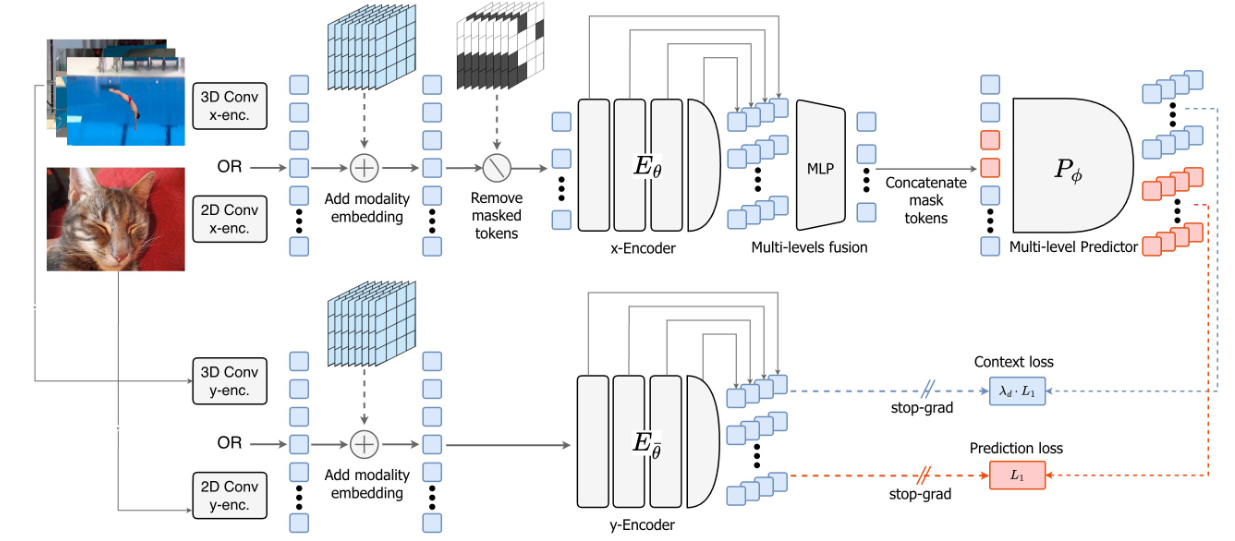
\includegraphics[width=\textwidth]{fig/vjepa2.png}
\caption{Architecture of V-JEPA~2.1 self-supervised pretraining framework showing the dual x-Encoder and y-Encoder pipeline with multi-level fusion, mask-denoising prediction, and stop-gradient targets \citep{murlabadia2026vjepa21}.}
\label{fig:vjepa2_arch}
\end{figure}

\subsubsection{Qwen2.5-VL (Alibaba Cloud)}

Qwen2.5-VL \citep{bai2025qwen2vl, qwen2025qwen3vl} is a 7-billion parameter autoregressive Vision-Language Model (VLM) that integrates visual understanding with language generation through cross-modal alignment. Unlike V-JEPA~2.1's purely visual self-supervised learning, Qwen2.5-VL acquires visual representations through joint training on massive image-text pairs and visual instruction tuning, producing features that are inherently grounded in linguistic semantics.

\paragraph{Vision Encoder and Native Dynamic Resolution.}
The Qwen2.5-VL Vision Encoder is a redesigned ViT trained from scratch to support \emph{native dynamic resolution} processing. Rather than resizing all inputs to a fixed resolution (e.g., $224 \times 224$), the encoder preserves the original aspect ratio and resolution of each input frame, partitioning it into non-overlapping patches of size $14 \times 14$ pixels. For video inputs, a 3D convolutional (Conv3D) patch embedding layer groups adjacent frames temporally (temporal stride of 2) to form spatiotemporal patches, reducing the total token count while preserving temporal context:
\begin{equation}
    \mathbf{v}_0 = \text{Conv3D}(\mathbf{V}_{\text{frames}}), \quad \mathbf{v}_0 \in \mathbb{R}^{N_v \times D_v}
    \label{eq:qwen_patchEmbed}
\end{equation}
where $N_v$ varies dynamically based on input resolution and $D_v$ is the vision encoder hidden dimension. This dynamic tokenization avoids information loss from aggressive resizing and produces a variable number of visual tokens per input.

\paragraph{Window Attention.}
To manage computational cost for high-resolution inputs, the Vision Encoder employs \emph{window attention} instead of global self-attention. Self-attention is computed locally within predefined spatial windows (e.g., $112 \times 112$ in patch space), reducing the computational complexity from $\mathcal{O}(N_v^2)$ to $\mathcal{O}(N_v \cdot w^2)$ where $w$ is the window size:
\begin{equation}
    \text{WindowAttn}(\mathbf{Q}, \mathbf{K}, \mathbf{V}) = \text{softmax}\!\left(\frac{\mathbf{Q}_w \mathbf{K}_w^T}{\sqrt{d_k}}\right) \mathbf{V}_w
    \label{eq:qwen_windowattn}
\end{equation}
where subscript $w$ denotes restriction to tokens within the same spatial window. This enables efficient processing of long video sequences without quadratic memory growth.

\paragraph{Multimodal Rotary Position Embedding (MRoPE).}
A key architectural innovation in Qwen2.5-VL is the \emph{Multimodal Rotary Position Embedding} (MRoPE), which extends the standard 1D RoPE used in language models to accommodate the multi-dimensional nature of visual inputs. The embedding dimension is decomposed into three segments, each encoding a separate positional axis---temporal ($t$), height ($h$), and width ($w$):
\begin{equation}
    \text{MRoPE}(\mathbf{x}, t, h, w) = \mathbf{x} \odot \left[\cos(\theta_t), \cos(\theta_h), \cos(\theta_w)\right] + \hat{\mathbf{x}} \odot \left[\sin(\theta_t), \sin(\theta_h), \sin(\theta_w)\right]
    \label{eq:qwen_mrope}
\end{equation}
where $\theta_t$, $\theta_h$, and $\theta_w$ are the rotation angles computed from the respective positional indices, and $\hat{\mathbf{x}}$ denotes the rotated complement of $\mathbf{x}$. For video inputs, the temporal position IDs are aligned with \emph{absolute time} rather than frame indices, enabling the model to learn the pace of events and perform temporal grounding at second-level precision. Notably, when all three positional indices are set equal ($t = h = w$), MRoPE reduces to standard 1D RoPE, ensuring compatibility with pure text decoding.

\paragraph{Visual-Language Fusion.}
After the Vision Encoder processes visual inputs, the resulting visual tokens are projected into the language model's embedding space through a multi-layer perceptron (MLP) merger:
\begin{equation}
    \mathbf{v}_{\text{lang}} = \text{MLP}_{\text{merge}}(\mathbf{v}_{\text{enc}}), \quad \mathbf{v}_{\text{lang}} \in \mathbb{R}^{N_v' \times D_{\text{LM}}}
    \label{eq:qwen_merge}
\end{equation}
where $D_{\text{LM}} = 3584$ is the hidden dimension of the Qwen2.5 language model decoder. The projected visual tokens are interleaved with text tokens to form a unified multimodal sequence, which is processed autoregressively by the Qwen2.5 LM Decoder. The model is trained to maximize the conditional log-likelihood of the next token:
\begin{equation}
    \mathcal{L}_{\text{LM}} = -\sum_{t=1}^{T_{\text{seq}}} \log p_\theta(x_t \mid x_{<t}, \mathbf{v}_{\text{lang}})
    \label{eq:qwen_lm_obj}
\end{equation}

\paragraph{4-bit NF4 Quantization.}
Due to GPU memory constraints (15.6~GB VRAM on the NVIDIA Tesla T4), Qwen2.5-VL is loaded in 4-bit NormalFloat (NF4) quantization with double quantization via the BitsAndBytes library. NF4 quantization maps full-precision weights $\mathbf{W} \in \mathbb{R}$ to a 4-bit data type optimized for normally distributed neural network weights:
\begin{equation}
    \mathbf{W}_{\text{NF4}} = \text{quantize}_{\text{NF4}}\!\left(\frac{\mathbf{W}}{s}\right) \cdot s, \quad s = \frac{\max(|\mathbf{W}_{\text{block}}|)}{q_{\max}}
    \label{eq:qwen_nf4}
\end{equation}
where $s$ is a per-block scaling factor and $q_{\max}$ is the maximum quantile value in the NF4 data type. Double quantization further compresses the scaling factors themselves to 8-bit, reducing the model memory footprint from approximately 14~GB (float16) to approximately 4~GB while preserving inference quality.

\paragraph{Feature Extraction Protocol.}
In this study, Qwen2.5-VL is used as a frozen feature extractor rather than a generative model. Four uniformly sampled frames per clip are processed through the Vision Encoder and LM Decoder via a minimal chat template prompt. The hidden states from the final decoder layer are mean-pooled across the sequence dimension to produce a single 3,584-dimensional embedding per clip:
\begin{equation}
    \mathbf{f}_{\text{Qwen}} = \frac{1}{T_{\text{seq}}} \sum_{t=1}^{T_{\text{seq}}} \mathbf{h}_t^{(L)}, \quad \mathbf{f}_{\text{Qwen}} \in \mathbb{R}^{3584}
    \label{eq:qwen_feat}
\end{equation}

\begin{figure}[H]
\centering
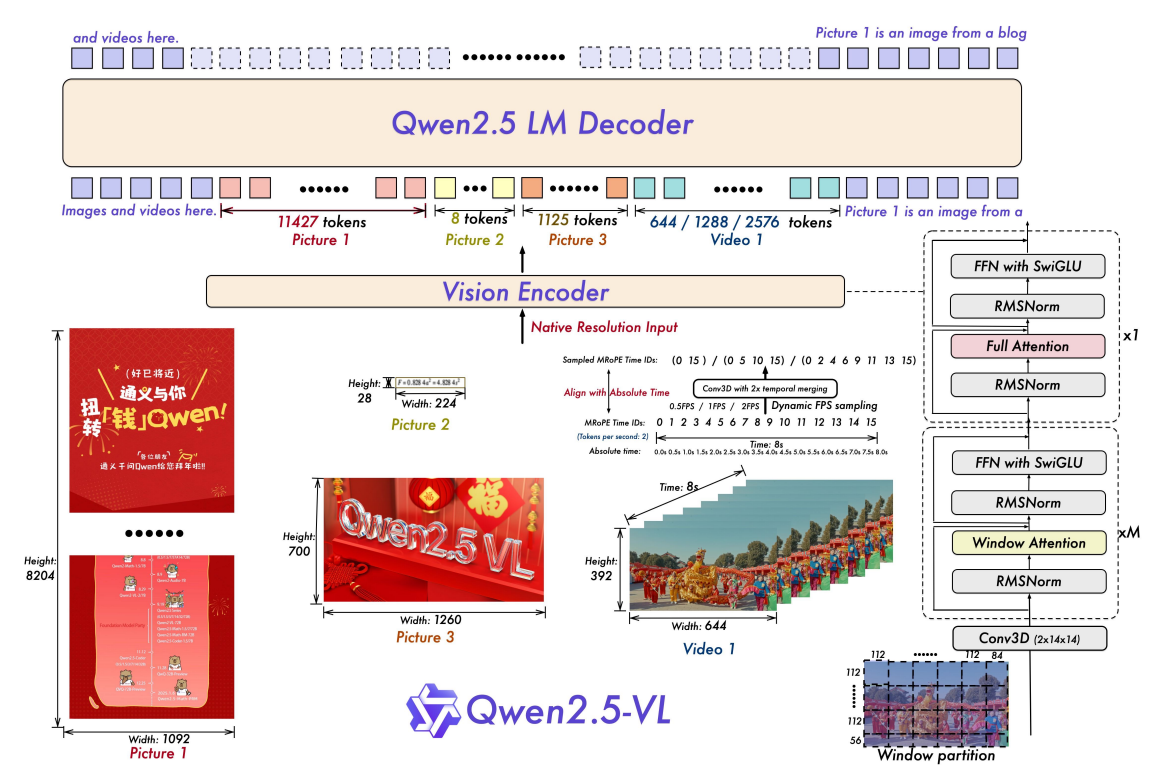
\includegraphics[width=\textwidth]{fig/qwen.png}
\caption{Architecture of Qwen2.5-VL vision-language model illustrating the Vision Encoder with Conv3D patch embedding, window attention, and native resolution input processing, feeding into the Qwen2.5 LM Decoder with MRoPE temporal alignment \citep{qwen2025qwen3vl}.}
\label{fig:qwen_arch}
\end{figure}


\section{Methods}

\subsection{Experimental Pipeline and Flowchart}

The experimental pipeline follows a structured sequence: video frame extraction, multi-layer feature vector extraction, standardization, dimensionality reduction via Principal Component Analysis (PCA), and multi-classifier evaluation including the novel HAF-STD Net architecture. Figure~\ref{fig:methodology_detailed} illustrates the pipeline.

\begin{figure}[p]
\centering
\vspace*{\fill}
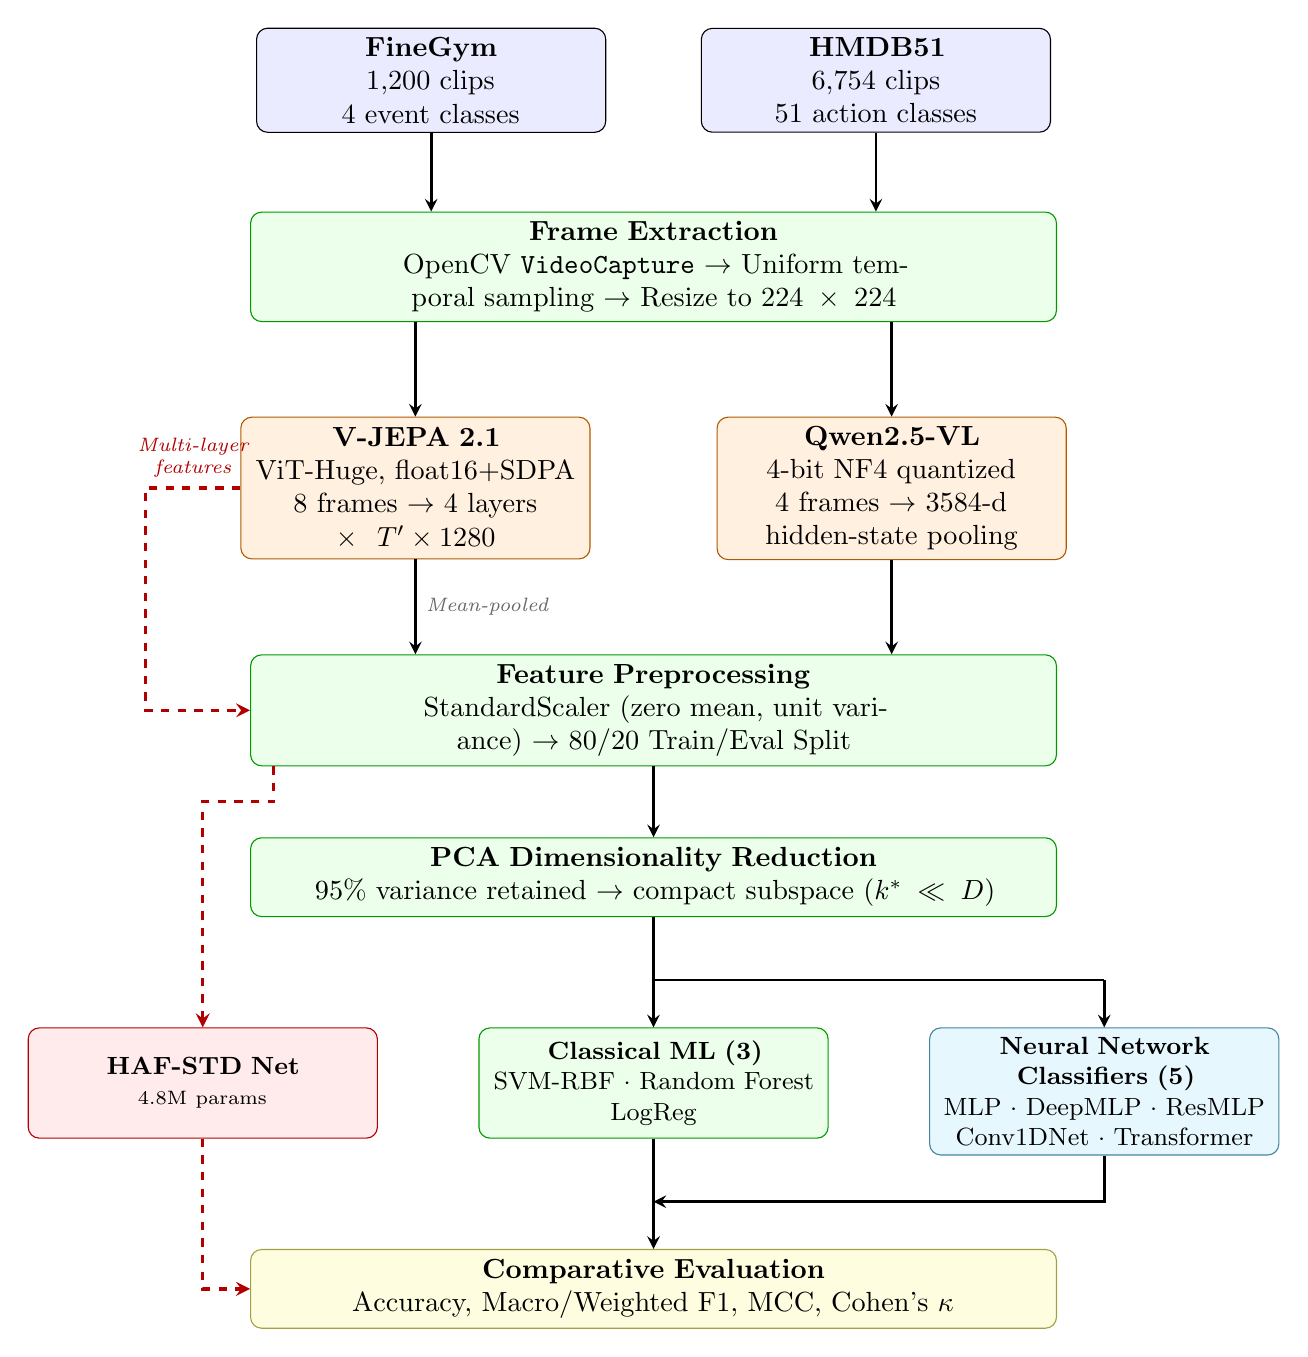
\begin{tikzpicture}[
    node distance=0.8cm,
    block/.style={rectangle, draw, fill=blue!8, text width=4.2cm, text centered, rounded corners, minimum height=1.0cm, font=\normalsize},
    modelblock/.style={rectangle, draw=orange!70!black, fill=orange!12, text width=4.2cm, text centered, rounded corners, minimum height=1.8cm, font=\normalsize},
    procblock/.style={rectangle, draw=green!60!black, fill=green!8, text width=10.0cm, text centered, rounded corners, minimum height=1.0cm, font=\normalsize},
    pcablock/.style={rectangle, draw=green!60!black, fill=green!8, text width=10.0cm, text centered, rounded corners, minimum height=1.0cm, font=\normalsize},
    branchblock/.style={rectangle, draw=green!60!black, fill=green!8, text width=4.2cm, text centered, rounded corners, minimum height=1.4cm, font=\small},
    trainblock/.style={rectangle, draw=cyan!60!black, fill=cyan!10, text width=4.2cm, text centered, rounded corners, minimum height=1.4cm, font=\small},
    novelblock/.style={rectangle, draw=red!70!black, fill=red!8, text width=4.2cm, text centered, rounded corners, minimum height=1.4cm, font=\small},
    resultblock/.style={rectangle, draw=yellow!60!black, fill=yellow!12, text width=10.0cm, text centered, rounded corners, minimum height=1.0cm, font=\normalsize},
    arrow/.style={->, >=stealth, thick, line width=1pt},
    redarrow/.style={->, >=stealth, thick, line width=1.2pt, dashed, red!70!black},
]
    % === Stage 1: Data Sources ===
    \node[block] (fg_src) {\textbf{FineGym}\\1,200 clips\\4 event classes};
    \node[block, right=1.2cm of fg_src] (hmdb_src) {\textbf{HMDB51}\\6,754 clips\\51 action classes};

    % === Stage 2: Frame Extraction ===
    \node[procblock, below=1.0cm of $(fg_src.south)!0.5!(hmdb_src.south)$] (frames) {\textbf{Frame Extraction}\\OpenCV \texttt{VideoCapture} $\rightarrow$ Uniform temporal sampling $\rightarrow$ Resize to $224\times224$};

    % === Stage 3: Feature Extractors ===
    \node[modelblock, below left=1.2cm and 0.8cm of frames.south] (vjepa) {\textbf{V-JEPA~2.1}\\ViT-Huge, float16+SDPA\\8 frames $\rightarrow$ 4 layers\\$\times\;T'\!\times\!1280$};
    \node[modelblock, below right=1.2cm and 0.8cm of frames.south] (qwen) {\textbf{Qwen2.5-VL}\\4-bit NF4 quantized\\4 frames $\rightarrow$ 3584-d\\hidden-state pooling};

    % === Stage 4a: Feature Preprocessing — StandardScaler (all classifiers) ===
    \node[procblock, below=1.2cm of $(vjepa.south)!0.5!(qwen.south)$] (scaler) {\textbf{Feature Preprocessing}\\StandardScaler (zero mean, unit variance) $\rightarrow$ 80/20 Train/Eval Split};

    % === Stage 4b: PCA Dimensionality Reduction (baseline classifiers only) ===
    \node[pcablock, below=0.9cm of scaler] (pca) {\textbf{PCA Dimensionality Reduction}\\95\% variance retained $\rightarrow$ compact subspace ($k^* \ll D$)};

    % === Stage 5: Classifier Branches ===
    % HAF-STD Net (far left — multi-layer features, uses StandardScaler but bypasses PCA)
    \node[novelblock, below left=1.4cm and 3.5cm of pca.south] (hafstd) {\textbf{HAF-STD Net}\\{\scriptsize 4.8M params}};
    % Classical ML (center — shared path, both models)
    \node[branchblock, below=1.4cm of pca] (classify_sk) {\textbf{Classical ML (3)}\\SVM-RBF $\cdot$ Random Forest\\LogReg};
    % Neural Network Baselines (right — shared path, both models)
    \node[trainblock, below right=1.4cm and 3.5cm of pca.south] (classify_pt) {\textbf{Neural Network Classifiers (5)}\\MLP $\cdot$ DeepMLP $\cdot$ ResMLP\\Conv1DNet $\cdot$ Transformer};

    % === Stage 6: Comparative Evaluation ===
    \node[resultblock, below=1.4cm of classify_sk] (results) {\textbf{Comparative Evaluation}\\Accuracy, Macro/Weighted F1, MCC, Cohen's $\kappa$};

    % ====== ARROWS ======

    % Data sources -> Frame extraction
    \draw[arrow] (fg_src.south) -- (fg_src.south |- frames.north);
    \draw[arrow] (hmdb_src.south) -- (hmdb_src.south |- frames.north);

    % Frame extraction -> Models
    \draw[arrow] (frames.south -| vjepa.north) -- (vjepa.north);
    \draw[arrow] (frames.south -| qwen.north) -- (qwen.north);

    % Models -> StandardScaler (mean-pooled features for baselines, multi-layer for HAF-STD)
    \draw[arrow] (vjepa.south) -- (vjepa.south |- scaler.north)
        node[midway, right, font=\scriptsize\itshape, text=black!60] {Mean-pooled};
    \draw[arrow] (qwen.south) -- (qwen.south |- scaler.north);

    % V-JEPA multi-layer features -> StandardScaler (HAF-STD path enters preprocessing)
    \draw[redarrow] (vjepa.west) -- node[above, font=\scriptsize\itshape, text=red!70!black, align=center] {Multi-layer\\features} ++(-1.2, 0) |- (scaler.west);

    % StandardScaler -> PCA (baseline path)
    \draw[arrow] (scaler.south) -- (pca.north);

    % StandardScaler -> HAF-STD Net (bypasses PCA)
    \draw[redarrow] (scaler.south west) ++(0.3,0) -- ++(0,-.45) -| (hafstd.north);

    % PCA -> Shared classifier branches (two-way fan)
    \coordinate (fan) at ($(pca.south) + (0,-0.8)$);
    \draw[thick] (pca.south) -- (fan);
    \draw[arrow] (fan) -- (classify_sk.north);
    \coordinate (above_pt) at (fan -| classify_pt.north);
    \draw[thick] (fan) -- (above_pt);
    \draw[arrow] (above_pt) -- (classify_pt.north);

    % Shared classifiers -> Comparative Evaluation (fan-in)
    \coordinate (merge) at ($(classify_sk.south) + (0,-0.8)$);
    \draw[thick] (classify_sk.south) -- (merge);
    \draw[arrow] (merge) -- (results.north);
    \draw[arrow] (classify_pt.south) |- (merge);

    % HAF-STD -> Comparative Evaluation (dashed red path along left side)
    \draw[redarrow] (hafstd.south) |- (results.west);

\end{tikzpicture}
\vspace*{\fill}
\caption{Methodology flowchart showing the experimental pipeline.}
\label{fig:methodology_detailed}
\end{figure}

\clearpage
\subsection{Frozen-Feature Protocol}

Under the frozen-feature protocol \citep{assran2023ijepa, assran2025vjepa2}, backbone model weights $\mathbf{\Theta}$ remain fixed throughout downstream training:
\begin{equation}
\mathbf{z}_i = f(\mathbf{x}_i; \mathbf{\Theta}_{\text{frozen}}), \quad \nabla_{\mathbf{\Theta}} \mathcal{L} = \mathbf{0}
\end{equation}
Only downstream classifier weights $\mathbf{W}_{\text{head}}$ are optimized:
\begin{equation}
\mathbf{W}_{\text{head}}^* = \arg\min_{\mathbf{W}_{\text{head}}} \frac{1}{N}\sum_{i=1}^{N} \mathcal{L}\left( g(\mathbf{z}_i; \mathbf{W}_{\text{head}}), y_i \right)
\end{equation}

\subsection{Feature Preprocessing and PCA Dimensionality Reduction}

Extracted raw feature representations $\mathbf{Z} \in \mathbb{R}^{N \times D}$ are first standardized to zero mean and unit variance using the training-split statistics:
\begin{equation}
\tilde{\mathbf{z}}_{ij} = \frac{z_{ij} - \mu_j}{\sigma_j}, \quad \mu_j = \frac{1}{N_{\text{train}}} \sum_{i=1}^{N_{\text{train}}} z_{ij}, \quad \sigma_j = \sqrt{\frac{1}{N_{\text{train}}-1} \sum_{i=1}^{N_{\text{train}}} (z_{ij} - \mu_j)^2}
\label{eq:standardization}
\end{equation}
where $j \in \{1, \ldots, D\}$ indexes feature dimensions. Standardization ensures that all features contribute equally to the subsequent dimensionality reduction step, preventing high-variance dimensions from dominating the principal component decomposition. The same $\mu_j$ and $\sigma_j$ statistics computed from the training split are applied to the test split to avoid data leakage.

Principal Component Analysis (PCA) is then applied to project the standardized features into a lower-dimensional, decorrelated subspace. Given the standardized feature matrix $\tilde{\mathbf{Z}} \in \mathbb{R}^{N \times D}$, PCA computes the covariance matrix:
\begin{equation}
\mathbf{C} = \frac{1}{N_{\text{train}}-1} \tilde{\mathbf{Z}}_{\text{train}}^\top \tilde{\mathbf{Z}}_{\text{train}} \in \mathbb{R}^{D \times D}
\label{eq:covariance}
\end{equation}
and performs eigendecomposition $\mathbf{C} = \mathbf{V} \boldsymbol{\Lambda} \mathbf{V}^\top$, where $\boldsymbol{\Lambda} = \text{diag}(\lambda_1, \lambda_2, \ldots, \lambda_D)$ contains eigenvalues sorted in descending order ($\lambda_1 \ge \lambda_2 \ge \cdots \ge \lambda_D \ge 0$) and $\mathbf{V} = [\mathbf{v}_1, \mathbf{v}_2, \ldots, \mathbf{v}_D]$ contains the corresponding orthonormal eigenvectors (principal components). The number of retained components $k^*$ is selected as the minimum $k$ that preserves at least 95\% of the total variance:
\begin{equation}
k^* = \arg\min_{k} \left( \frac{\sum_{j=1}^{k} \lambda_j}{\sum_{j=1}^{D} \lambda_j} \ge 0.95 \right)
\label{eq:pca_k}
\end{equation}
The projection onto the retained subspace is then given by:
\begin{equation}
\mathbf{Z}_{\text{PCA}} = \tilde{\mathbf{Z}} \, \mathbf{V}_{:k^*} \in \mathbb{R}^{N \times k^*}
\label{eq:pca_projection}
\end{equation}
where $\mathbf{V}_{:k^*} \in \mathbb{R}^{D \times k^*}$ contains the first $k^*$ principal components.

The 95\% variance retention threshold was chosen as a standard balance between information preservation and dimensionality reduction. On the FineGym dataset, PCA reduced V-JEPA~2.1 features from $D=1{,}280$ to $k^*=90$ dimensions and Qwen2.5-VL features from $D=3{,}584$ to $k^*=142$ dimensions. On HMDB51, V-JEPA~2.1 features were reduced to $k^*=286$ and Qwen2.5-VL features to $k^*=719$ dimensions. The substantially higher retained dimensionality for HMDB51 reflects the greater representational complexity required to distinguish 51 action classes compared to FineGym's 4 classes.

PCA serves three key purposes in this pipeline: (1)~it decorrelates features, removing redundant collinear dimensions that arise from the over-parameterized encoder architectures; (2)~it reduces computational cost for the classical ML classifiers (SVM-RBF, Random Forest), which scale poorly with high-dimensional inputs; and (3)~it mitigates the curse of dimensionality, particularly for the smaller FineGym dataset where the sample-to-feature ratio would otherwise be unfavourable. Importantly, PCA is applied \textit{only} to the baseline classifier pathway. The HAF-STD Net receives the full-dimensional, multi-layer temporal tensor without PCA reduction, as its spectral-temporal decomposition module (Section~\ref{sec:hafstd_net}) operates directly on the spatiotemporal structure and benefits from preserving the complete representational capacity.


\subsection{Classifier Architectures}

Extracted features are evaluated across 8 baseline classifiers plus the HAF-STD Net architecture (9 classifiers total):

\subsubsection{Classical Machine Learning Classifiers}

\begin{enumerate}[leftmargin=*]
    \item \textbf{Support Vector Machine (SVM-RBF)} \citep{cortes1995svm}\textbf{:} Radial Basis Function kernel $K(\mathbf{x}_i, \mathbf{x}_j) = \exp\left(-\gamma \|\mathbf{x}_i - \mathbf{x}_j\|^2\right)$ with $C=1.0$.
    \item \textbf{Random Forest} \citep{breiman2001randomforests}\textbf{:} Ensemble of 500 decision trees with balanced class weighting.
    \item \textbf{Logistic Regression} \citep{cox1958logistic}\textbf{:} Linear probe with L2 regularization ($C=1.0$) and multinomial softmax.
\end{enumerate}

\subsubsection{Neural Network Classifiers}

\begin{enumerate}[leftmargin=*]
    \item \textbf{Multi-Layer Perceptron (MLP)} \citep{rumelhart1986backprop}\textbf{:} Scikit-learn MLP with 2 hidden layers (512, 256), ReLU, and Adam optimizer.
    \item \textbf{DeepMLP:} 4-layer feedforward network (Input $\rightarrow$ 512 $\rightarrow$ 256 $\rightarrow$ 128 $\rightarrow$ Classes) with BatchNorm \citep{ioffe2015batchnorm}, ReLU, and Dropout \citep{srivastava2014dropout} (0.3).
    \item \textbf{ResMLP} \citep{he2016resnet}\textbf{:} Deep residual MLP with skip connections: $\mathbf{h}_{l+1} = \mathbf{h}_l + \mathcal{F}(\mathbf{h}_l, \mathbf{W}_l)$.
    \item \textbf{Conv1DNet} \citep{lecun1998cnn}\textbf{:} 1D Convolutional network projecting feature dimension as spatial channels followed by adaptive max pooling.
    \item \textbf{MiniTransformer} \citep{vaswani2017attention}\textbf{:} Self-Attention transformer encoder block with multi-head attention ($h=4$) and feedforward projection.
\end{enumerate}

\subsubsection{HAF-STD Net Classifier}
\label{sec:hafstd_net}

We propose \textbf{HAF-STD Net} (Hierarchical Adaptive Fusion with Spectral-Temporal Decomposition), a specialized classification architecture that jointly exploits V-JEPA~2.1's unique properties of temporal coherence and deep self-supervision. The architecture contains 4.8M trainable parameters and operates on multi-layer per-frame features extracted from the frozen V-JEPA~2.1 encoder. HAF-STD Net introduces three core components:

\paragraph{1. Spectral-Temporal Decomposition via Haar DWT.}
A 1D Haar Discrete Wavelet Transform is applied along the temporal axis of V-JEPA~2.1's latent token sequences at each selected encoder layer. This decomposes the temporal signal into low-frequency (appearance/trend) and high-frequency (motion/change dynamics) components:
\begin{equation}
\mathbf{a}_k = \frac{1}{2}(\mathbf{h}_{2t} + \mathbf{h}_{2t+1}), \quad
\mathbf{d}_k = \frac{1}{2}(\mathbf{h}_{2t} - \mathbf{h}_{2t+1})
\end{equation}
where $\mathbf{a}_k$ captures static appearance and $\mathbf{d}_k$ captures motion dynamics at layer $k$. The mean-pooled approximation and detail coefficients form the \emph{appearance stream} and \emph{motion stream}, respectively.

\paragraph{2. Depth Representation Velocity.}
Inter-layer deltas are computed between consecutive selected encoder layers:
\begin{equation}
\Delta\mathbf{H}_k = \bar{\mathbf{H}}_{k+1} - \bar{\mathbf{H}}_k, \quad k \in \{1, 2, 3\}
\end{equation}
where $\bar{\mathbf{H}}_k$ denotes the temporally mean-pooled hidden state at layer $k$. These \emph{velocity vectors} capture how the model's internal understanding progressively transforms across its depth---a signal that is action-class-dependent due to V-JEPA~2.1's deep self-supervision training. Between the 4 selected layers, there are exactly $4 - 1 = 3$ consecutive inter-layer velocity vectors.

\paragraph{3. Adaptive Routing over Depth $\times$ Frequency Streams.}
The decomposed streams across layers (4 appearance streams, 4 motion streams, and 3 depth velocity streams) are independently projected through dedicated linear heads, yielding $4 + 4 + 3 = 11$ feature vectors. An adaptive routing network learns input-dependent fusion weights:
\begin{equation}
\mathbf{w} = \text{softmax}\left(\text{MLP}\left([\mathbf{s}_1; \mathbf{s}_2; \ldots; \mathbf{s}_{11}]\right)\right), \quad
\mathbf{f} = \sum_{i=1}^{11} w_i \cdot \mathbf{s}_i
\end{equation}
The fused representation $\mathbf{f}$ is classified via a cosine similarity head with learnable temperature scaling $\tau$:
\begin{equation}
p(y=c | \mathbf{f}) = \frac{\exp\left(\tau \cdot \hat{\mathbf{f}}^T \hat{\mathbf{w}}_c\right)}{\sum_{j=1}^{C} \exp\left(\tau \cdot \hat{\mathbf{f}}^T \hat{\mathbf{w}}_j\right)}
\end{equation}

\begin{figure}[H]
\centering
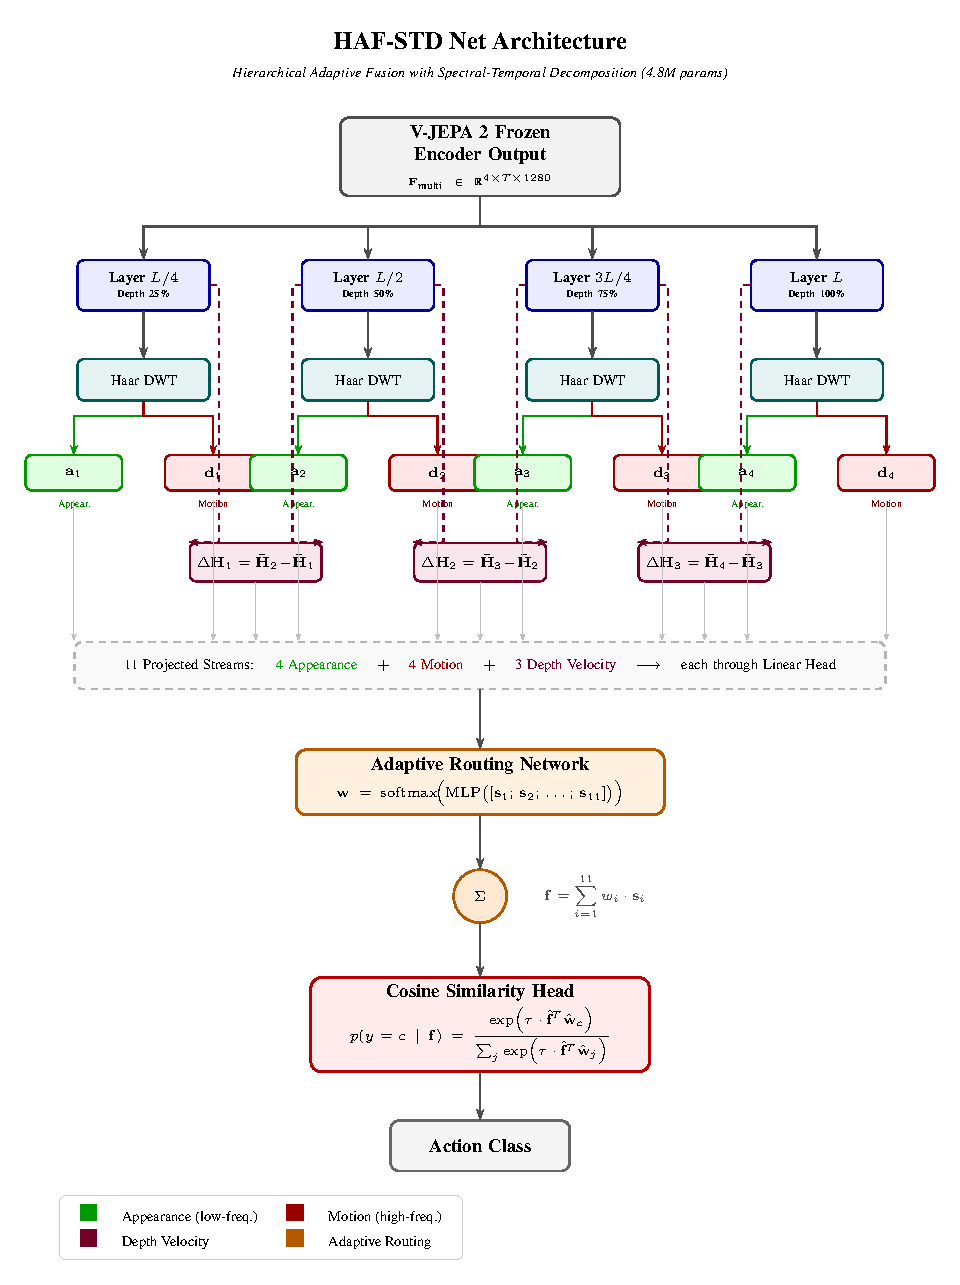
\includegraphics[width=\textwidth]{fig/hafstd_figure.pdf}
\caption{Architecture of the proposed HAF-STD Net classifier.}
\label{fig:hafstd_arch}
\end{figure}

\subsection{Training Techniques and Optimization}

All neural network classifiers are trained using:
\begin{itemize}[leftmargin=*]
    \item \textbf{Label Smoothing ($\epsilon = 0.1$):} Softens one-hot target vectors $y_c^{\text{smooth}} = (1 - \epsilon) y_c + \frac{\epsilon}{C}$.
    \item \textbf{Feature-Space Mixup ($\alpha = 0.2$):} Interpolates feature pairs: $\tilde{\mathbf{z}} = \lambda \mathbf{z}_i + (1-\lambda)\mathbf{z}_j$.
    \item \textbf{Cosine Annealing LR:} Learning rate schedule decaying from $10^{-3}$ to $10^{-6}$.
    \item \textbf{Optimizer:} AdamW with weight decay $\lambda=10^{-4}$.
    \item \textbf{Early Stopping:} Triggers after 15 epochs without validation loss improvement.
\end{itemize}

\subsection{Evaluation Metrics}
\label{sec:eval_metrics}

To thoroughly assess classification performance and mitigate potential biases arising from class imbalance or superficial prediction heuristics, model evaluation is grounded on a comprehensive suite of quantitative metrics. In this study, experiments encompass both fine-grained action classification on FineGym ($C = 4$ sub-action categories) and coarse-grained classification across diverse motion categories on HMDB51 ($C = 51$ classes).

\subsubsection{Confusion Matrix and Multi-Class Decomposition}

All evaluated metrics are derived from the empirical confusion matrix $\mathbf{M} \in \mathbb{N}^{C \times C}$, where each element $M_{ij}$ denotes the count of test samples whose true ground-truth class is $i$ but were classified into class $j$ by the model. The total number of evaluation samples is given by $N = \sum_{i=1}^{C}\sum_{j=1}^{C} M_{ij}$.

For any individual target class $c \in \{1, 2, \dots, C\}$, multi-class evaluation can be decomposed into a set of binary One-vs-Rest (OvR) classification problems using four fundamental quantities:
\begin{itemize}[leftmargin=*]
    \item \textbf{True Positives ($TP_c$):} The number of video instances correctly predicted as class $c$:
    \begin{equation}
    TP_c = M_{cc}
    \end{equation}
    \item \textbf{False Positives ($FP_c$):} The number of video instances belonging to classes other than $c$ that are incorrectly predicted as class $c$ (Type I error / false alarm):
    \begin{equation}
    FP_c = \sum_{i \neq c} M_{ic}
    \end{equation}
    \item \textbf{False Negatives ($FN_c$):} The number of video instances belonging to true class $c$ that are incorrectly assigned to a different class (Type II error / missed detection):
    \begin{equation}
    FN_c = \sum_{j \neq c} M_{cj}
    \end{equation}
    \item \textbf{True Negatives ($TN_c$):} The number of video instances not belonging to class $c$ that are correctly predicted as non-$c$:
    \begin{equation}
    TN_c = \sum_{i \neq c} \sum_{j \neq c} M_{ij} = N - TP_c - FP_c - FN_c
    \end{equation}
\end{itemize}
The total ground-truth support (number of true instances) for class $c$ is defined as $N_c = TP_c + FN_c = \sum_{j=1}^C M_{cj}$, while the total number of predictions assigned to class $c$ is $P_c = TP_c + FP_c = \sum_{i=1}^C M_{ic}$.

\subsubsection{Classification Accuracy}

Overall classification accuracy measures the fraction of all test video clips whose top predicted class label coincides with the ground-truth annotation:
\begin{equation}
\text{Accuracy} = \frac{\sum_{c=1}^{C} M_{cc}}{N} = \frac{1}{N}\sum_{i=1}^{N} \mathbf{1}\left(\hat{y}_i = y_i\right)
\end{equation}
where $\hat{y}_i = \arg\max_c \, p(y=c \mid \mathbf{x}_i)$ is the model's highest-probability predicted class for sample $\mathbf{x}_i$, $y_i$ is the corresponding ground-truth label, and $\mathbf{1}(\cdot)$ is the indicator function. 

In single-label multi-class video classification, this is standard overall accuracy (top-1 decision rule). Under uniform random chance, the expected accuracy corresponds to $1/C$, yielding $25.0\%$ for FineGym ($C = 4$) and approximately $1.96\%$ for HMDB51 ($C = 51$). While overall accuracy provides an intuitive global benchmark of model correctness, it weights all instances equally and can thus be dominated by high-support majority classes. Consequently, additional class-balanced and chance-adjusted metrics are required.

\subsubsection{Precision (Macro and Weighted)}

Precision assesses the reliability or purity of model predictions for a given category. For class $c$, it represents the probability that a sample predicted to be class $c$ truly belongs to class $c$:
\begin{equation}
\text{Precision}_c = \frac{TP_c}{TP_c + FP_c} = \frac{M_{cc}}{\sum_{i=1}^{C} M_{ic}}
\end{equation}
High precision indicates that when the classifier predicts an action, the prediction has a low rate of false alarms. To summarize precision across all $C$ classes, two aggregation schemes are reported:
\begin{itemize}[leftmargin=*]
    \item \textbf{Macro-Averaged Precision:} The unweighted arithmetic mean across all per-class precisions:
    \begin{equation}
    \text{Precision}_{\text{macro}} = \frac{1}{C}\sum_{c=1}^{C} \text{Precision}_c
    \end{equation}
    Macro precision assigns equal importance to every class regardless of class support size, strictly highlighting models that misclassify smaller or more ambiguous classes.
    \item \textbf{Weighted Precision:} The support-weighted average of per-class precisions:
    \begin{equation}
    \text{Precision}_{\text{weighted}} = \sum_{c=1}^{C} \frac{N_c}{N} \, \text{Precision}_c
    \end{equation}
\end{itemize}

\subsubsection{Recall / Sensitivity (Macro and Weighted)}

Recall (also known as true positive rate or sensitivity) measures the completeness of detection for a given class. For class $c$, it indicates the proportion of true class $c$ video instances that the model successfully retrieves:
\begin{equation}
\text{Recall}_c = \frac{TP_c}{TP_c + FN_c} = \frac{M_{cc}}{\sum_{j=1}^{C} M_{cj}} = \frac{M_{cc}}{N_c}
\end{equation}
High recall reflects that the model rarely misses actual instances of the specified action. The aggregated multi-class recall variants are computed as:
\begin{itemize}[leftmargin=*]
    \item \textbf{Macro-Averaged Recall:} The unweighted arithmetic average of per-class recalls:
    \begin{equation}
    \text{Recall}_{\text{macro}} = \frac{1}{C}\sum_{c=1}^{C} \text{Recall}_c
    \end{equation}
    \item \textbf{Weighted Recall:} The support-weighted average of class recalls:
    \begin{equation}
    \text{Recall}_{\text{weighted}} = \sum_{c=1}^{C} \frac{N_c}{N} \, \text{Recall}_c = \frac{\sum_{c=1}^{C} M_{cc}}{N} = \text{Accuracy}
    \end{equation}
    In single-label multi-class evaluation, weighted recall is mathematically identical to overall classification accuracy.
\end{itemize}

\subsubsection{F1-Score (Macro and Weighted)}

Because precision and recall frequently exhibit an inverse trade-off, the F1-score provides a balanced harmonic mean between the two measures. For class $c$, it is defined as:
\begin{equation}
F1_c = 2 \cdot \frac{\text{Precision}_c \cdot \text{Recall}_c}{\text{Precision}_c + \text{Recall}_c} = \frac{2 TP_c}{2 TP_c + FP_c + FN_c}
\end{equation}
The harmonic mean ensures that if either precision or recall is low for a given category, the corresponding $F1_c$ is heavily penalized. Multi-class aggregation is performed as follows:
\begin{itemize}[leftmargin=*]
    \item \textbf{Macro F1-Score:} The unweighted arithmetic average of individual class F1-scores:
    \begin{equation}
    F1_{\text{macro}} = \frac{1}{C}\sum_{c=1}^{C} F1_c
    \end{equation}
    Throughout this thesis, Macro F1 is treated as the primary ranking metric because it treats every action category with equal priority. A model cannot achieve a high Macro F1 score by solely predicting dominant classes while neglecting fine-grained or difficult minority classes.
    \item \textbf{Weighted F1-Score:} The support-weighted mean of per-class F1-scores:
    \begin{equation}
    F1_{\text{weighted}} = \sum_{c=1}^{C} \frac{N_c}{N} \, F1_c
    \end{equation}
\end{itemize}

\subsubsection{Matthews Correlation Coefficient (MCC)}

The Matthews Correlation Coefficient (MCC) is widely considered one of the most reliable and statistically sound omnibus metrics for classification. Unlike accuracy or individual F1 formulations that only focus on subset cells of the confusion matrix, MCC utilizes all elements of the confusion matrix symmetrically. Originally formulated for binary classification, MCC was generalized to the multi-class case ($C > 2$) by Gorodkin through covariance analysis of categorical vectors:
\begin{equation}
\label{eq:mcc_multiclass}
\text{MCC} = \frac{c \cdot N - \sum_{k=1}^{C} P_k \, N_k}{\sqrt{\left(N^2 - \sum_{k=1}^{C} P_k^2\right) \left(N^2 - \sum_{k=1}^{C} N_k^2\right)}}
\end{equation}
where:
\begin{itemize}[leftmargin=*]
    \item $c = \sum_{k=1}^{C} M_{kk}$ is the total number of correctly classified video clips,
    \item $N$ is the total number of test samples,
    \item $P_k = \sum_{i=1}^{C} M_{ik}$ is the total number of times class $k$ was predicted (column sum $k$),
    \item $N_k = \sum_{j=1}^{C} M_{kj}$ is the total number of ground-truth occurrences of class $k$ (row sum $k$).
\end{itemize}
MCC generates a correlation coefficient bounded strictly in the interval $[-1.0, +1.0]$:
\begin{itemize}[leftmargin=*]
    \item $\text{MCC} = +1.0$: Represents perfect prediction agreement where every test sample is correctly identified.
    \item $\text{MCC} = 0.0$: Represents prediction performance no better than random guessing based on marginal class distributions.
    \item $\text{MCC} = -1.0$: Represents complete inverse classification (total disagreement).
\end{itemize}
A fundamental advantage of MCC is that a trivial classifier (such as one that always predicts the majority class) yields an MCC of $0.0$, whereas overall accuracy would report misleadingly high scores.

\subsubsection{Cohen's Kappa ($\kappa$)}

Cohen's Kappa ($\kappa$) is a chance-adjusted measure of inter-rater agreement adapted for machine learning classification, where the classifier's predictions and the true ground-truth annotations are treated as two independent raters:
\begin{equation}
\label{eq:cohen_kappa}
\kappa = \frac{p_o - p_e}{1 - p_e}
\end{equation}
where:
\begin{itemize}[leftmargin=*]
    \item $p_o$ is the observed empirical agreement, equivalent to overall classification accuracy:
    \begin{equation}
    p_o = \frac{1}{N}\sum_{c=1}^{C} M_{cc}
    \end{equation}
    \item $p_e$ is the hypothetical probability of agreement occurring purely by chance, computed from the product of marginal distribution proportions:
    \begin{equation}
    p_e = \frac{1}{N^2}\sum_{c=1}^{C} P_c \cdot N_c = \sum_{c=1}^{C} \left(\frac{\sum_{i=1}^{C} M_{ic}}{N}\right) \left(\frac{\sum_{j=1}^{C} M_{cj}}{N}\right)
    \end{equation}
\end{itemize}
The metric normalizes observed accuracy against the baseline chance level $p_e$. Values of $\kappa$ range between $-1.0$ and $+1.0$, typically interpreted according to the standard Landis and Koch agreement scale:
\begin{itemize}[leftmargin=*]
    \item $\kappa < 0.00$: Poor agreement (worse than random chance).
    \item $0.00 \le \kappa \le 0.20$: Slight agreement.
    \item $0.21 \le \kappa \le 0.40$: Fair agreement.
    \item $0.41 \le \kappa \le 0.60$: Moderate agreement.
    \item $0.61 \le \kappa \le 0.80$: Substantial agreement.
    \item $0.81 \le \kappa \le 1.00$: Almost perfect agreement.
\end{itemize}
While MCC originates from Pearson correlation and treats confusion errors symmetrically in continuous Euclidean vector space, Cohen's Kappa originates from categorical agreement statistics. Reporting both metrics alongside Macro F1 provides mutually reinforcing validation that observed performance gains reflect genuine representational superiority rather than statistical artifacts.

\section{Tools and Techniques}

\subsection{Hardware Environment}

\begin{table}[H]
\centering
\caption{Hardware configuration for experiments.}
\label{tab:hardware_config}
\begin{tabular}{ll}
\toprule
\textbf{Component} & \textbf{Specification} \\
\midrule
GPU & NVIDIA Tesla T4 (15.6 GB VRAM) \\
CPU & Intel Xeon (2 cores) \\
RAM & 13 GB System Memory \\
Platform & Kaggle Notebooks \\
CUDA Version & 12.x \\
Persistent Storage & \texttt{/kaggle/working/} (saved as output) \\
\bottomrule
\end{tabular}
\end{table}

The NVIDIA Tesla T4 GPU, based on the Turing architecture, provides 15.6 GB of VRAM with support for mixed-precision (FP16) and INT8/INT4 operations. While not sufficient to load Qwen2.5-VL at full precision (which requires approximately 14 GB in float16), the T4 supports 4-bit quantization through the BitsAndBytes library, enabling deployment of the 7B-parameter model within the available memory budget.

\subsection{Software Stack}

\begin{table}[H]
\centering
\caption{Software libraries and their roles in the experimental pipeline.}
\label{tab:software_stack}
\begin{tabularx}{\textwidth}{l l X}
\toprule
\textbf{Library} & \textbf{Version} & \textbf{Purpose} \\
\midrule
Python & 3.12.13 & Programming language \\
PyTorch & 2.x (Latest) & Deep learning framework, CUDA backend, custom NN classifiers \\
Transformers & Latest & Hugging Face model hub, V-JEPA 2.1 and Qwen2.5-VL loading \\
BitsAndBytes & Latest & 4-bit NF4 quantization for Qwen2.5-VL \\
scikit-learn & Latest & Classical ML classifiers, PCA, metrics \\
OpenCV & Latest & Video frame extraction (\texttt{cv2.VideoCapture}) \\
yt-dlp & Latest & YouTube video downloading with temporal trimming \\
huggingface\_hub & Latest & HMDB51 dataset download (\texttt{hf\_hub\_download}) \\
NumPy & Latest & Numerical operations, frame indexing \\
Pillow (PIL) & Latest & Image format conversion \\
\bottomrule
\end{tabularx}
\end{table}

\subsection{Model Specifications}

\begin{table}[H]
\centering
\caption{Architectural specifications of V-JEPA 2.1 and Qwen2.5-VL.}
\label{tab:model_specs}
\begin{tabularx}{\textwidth}{l X X}
\toprule
\textbf{Specification} & \textbf{V-JEPA 2.1} & \textbf{Qwen2.5-VL} \\
\midrule
Parameters & 654M & 7B \\
Architecture & ViT-Huge & Qwen2.5 + ViT \\
Paradigm & Self-supervised (JEPA) & Autoregressive VLM \\
Pretraining & Masked latent prediction & Image-text pairs + instruction tuning \\
Input Frames & 8 & 4 \\
Input Resolution & $224 \times 224$ & Dynamic resolution \\
Feature Dimension & 1,280 & 3,584 \\
Precision & float16 + SDPA & 4-bit NF4 \\
Modality & Video only & Vision + Language \\
Hugging Face ID & \nolinkurl{facebook/vjepa2-vith-fpc64-256} & \nolinkurl{Qwen/Qwen2.5-VL-7B-Instruct} \\
\bottomrule
\end{tabularx}
\end{table}

\section{Implementation Details}

All experiments were implemented as Kaggle Notebooks executing on the cloud platform described in Section~3.3. The complete source code for all pipeline components is provided in Appendix~\ref{app:source_code}. This section describes the design rationale, algorithmic strategies, and key implementation decisions for each stage of the experimental pipeline.

\subsection{FineGym Data Pipeline}

The FineGym data acquisition pipeline is driven by the official annotation file, which provides YouTube video identifiers paired with precise event-level timestamps (start and end times) for each gymnastic routine. The pipeline operates in three stages:

\begin{enumerate}[leftmargin=*]
    \item Annotation Parsing: The annotation JSON is parsed to extract YouTube video IDs, event categories (BB, FX, UB, VT), and temporal boundaries for each event segment. A balanced sampling strategy selects 300 clips per apparatus category, yielding 1,200 total clips with uniform class distribution.
    
    \item Temporal Clip Extraction: Each event clip is downloaded from YouTube using \texttt{yt-dlp} with the \nolinkurl{--download-sections} flag and \nolinkurl{--force-keyframes-at-cuts} to ensure precise temporal trimming aligned to the annotation timestamps. The \nolinkurl{worst[ext=mp4]/worst} format selector downloads the lowest available quality to minimize bandwidth and storage while preserving sufficient visual information for subsequent frame extraction at $224 \times 224$ resolution (Listing~\ref{lst:fg_download} in Appendix~\ref{app:source_code}).
    
    \item Fault-Tolerant Execution: A JSON-based progress log tracks the download status of each clip, enabling the pipeline to resume after interruptions (e.g., Kaggle session timeouts or transient network errors) without re-downloading previously acquired clips. Each download is attempted up to 2 times with a 120-second timeout per attempt.
\end{enumerate}

\subsection{HMDB51 Data Pipeline}

The HMDB51 dataset was obtained as a 2.12~GB zip archive from the Hugging Face Hub (\texttt{jili5044/hmdb51}) using the \texttt{hf\_hub\_download} API. The standard Hugging Face \texttt{datasets}  archive was directly downloaded and extracted locally (Listing~\ref{lst:hmdb_download} in Appendix~\ref{app:source_code}).

After extraction, the pipeline constructs a sample index by recursively walking the directory tree. Action class labels are inferred from parent folder names, which follow HMDB51's standard directory-per-class organization. This process successfully loads all 6,754 video clips across 51 action categories with zero indexing errors. The directory-based approach provides reliable, schema-independent dataset loading that is robust to metadata inconsistencies in third-party repository mirrors.

\subsection{Feature Extraction Pipeline}

Feature extraction follows the frozen-feature protocol described in Section~3.2.2, where backbone model weights remain fixed and only downstream classifier parameters are trained. Both V-JEPA~2.1 and Qwen2.5-VL are loaded sequentially (one at a time) to manage GPU memory constraints within the 15.6~GB VRAM budget of the NVIDIA Tesla T4.

\subsubsection{V-JEPA~2.1 Feature Extraction}

V-JEPA~2.1 is loaded in float16 precision with Scaled Dot-Product Attention (SDPA) via the Hugging Face \texttt{transformers} library. For each video clip, 8 frames are uniformly sampled and resized to $224 \times 224$ pixels using the official \texttt{VJEPA2VideoProcessor}. The processed frames are passed through the frozen encoder under \texttt{torch.no\_grad()} with mixed-precision autocast to minimize GPU memory consumption. For baseline classifiers, the final-layer hidden states are spatially mean-pooled to produce a single 1,280-dimensional feature vector per clip (Equation~\ref{eq:qwen_feat}). For HAF-STD Net, hidden states are extracted from 4 intermediate encoder layers and spatially pooled per frame to produce the 4D multi-layer tensor $\mathbf{F}_{\text{multi}} \in \mathbb{R}^{4 \times T' \times 1280}$ (Equation~\ref{eq:vjepa_multilayer}). The complete extraction procedure is provided in Listing~\ref{lst:vjepa_extraction} (Appendix~\ref{app:source_code}).

\subsubsection{Qwen2.5-VL Feature Extraction}

After V-JEPA~2.1 extraction completes, the model is explicitly deleted from GPU memory, CUDA cache is cleared, and Python garbage collection is triggered before loading Qwen2.5-VL. The 7B-parameter model is loaded in 4-bit NF4 quantization (Equation~\ref{eq:qwen_nf4}) with double quantization enabled, reducing the model footprint from approximately 14~GB to approximately 4~GB.

Feature extraction from Qwen2.5-VL requires constructing a chat-template-formatted input for each video clip, as the model is designed for conversational visual question answering rather than direct feature extraction. A minimal prompt (``Describe.'') is applied to 4 uniformly sampled frames per clip. The model processes this multimodal input through its Vision Encoder and LM Decoder, and the hidden states from the final decoder layer are mean-pooled across the sequence dimension to produce a 3,584-dimensional feature vector per clip (Equation~\ref{eq:qwen_feat}). The full quantized extraction procedure is provided in Listing~\ref{lst:qwen_extraction} (Appendix~\ref{app:source_code}).

\subsection{Classifier Training Pipeline}

\subsubsection{Classical Machine Learning Classifiers}

The three scikit-learn classifiers (SVM-RBF, Random Forest, Logistic Regression) operate on PCA-reduced features and are trained using their default scikit-learn API with the hyperparameters specified in Section~3.2.4. These classifiers require no iterative training loop and are fitted in a single pass on the training split.

\subsubsection{Neural Network Classifiers}

The five neural network classifiers (MLP, DeepMLP, ResMLP, Conv1DNet, MiniTransformer) share a common training harness that implements the regularization techniques described in Section~3.2.5. The training procedure operates as follows:

\begin{enumerate}[leftmargin=*]
    \item \textbf{Optimization:} All models are trained with AdamW optimizer ($\text{lr} = 10^{-3}$, weight decay $= 10^{-4}$) and Cosine Annealing learning rate scheduling that decays the learning rate from $10^{-3}$ to $10^{-6}$ over the training horizon.
    
    \item \textbf{Feature-Space Mixup:} At each training step, input feature vectors are interpolated with randomly permuted counterparts using a mixing coefficient $\lambda \sim \text{Beta}(0.2, 0.2)$, clamped to $\lambda \geq 0.5$ to ensure the original sample dominates. The cross-entropy loss is computed as a weighted combination over both original and permuted labels.
    
    \item \textbf{Label Smoothing:} The one-hot target vectors are softened with $\epsilon = 0.1$, distributing $\frac{\epsilon}{C}$ probability mass to each non-target class to prevent over-confident predictions and improve calibration.
    
    \item \textbf{Early Stopping:} Training terminates after 15 consecutive epochs (30 for HAF-STD Net) without improvement in validation accuracy. The model checkpoint with the highest validation accuracy is restored as the final model.
\end{enumerate}

The ResMLP architecture (Listing~\ref{lst:resmlp_arch}) and the shared training loop (Listing~\ref{lst:training_loop}) are provided in Appendix~\ref{app:source_code}.

\subsubsection{HAF-STD Net Training}

The HAF-STD Net training pipeline extends the baseline training harness to accommodate the 4D multi-layer temporal tensor input $\mathbf{F}_{\text{multi}} \in \mathbb{R}^{B \times 4 \times T \times 1280}$. Unlike the baseline classifiers that operate on 1D PCA-reduced feature vectors, HAF-STD Net requires the full-dimensional multi-layer representation without PCA reduction, as the spectral-temporal decomposition and depth velocity computation (Section~\ref{sec:hafstd_net}) operate directly on the spatiotemporal structure.

The feature-space mixup augmentation is generalized to 4D tensors by applying element-wise interpolation across all dimensions simultaneously:
\begin{equation}
    \tilde{\mathbf{F}} = \lambda \cdot \mathbf{F}_i + (1 - \lambda) \cdot \mathbf{F}_{\pi(i)}, \quad \lambda \sim \text{Beta}(0.2, 0.2)
\end{equation}
where $\pi$ denotes a random permutation of the batch indices. This preserves the multi-layer temporal structure while providing regularization equivalent to the baseline mixup. The complete HAF-STD Net architecture (Listing~\ref{lst:hafstd_arch}) and training harness (Listing~\ref{lst:hafstd_train}) are provided in Appendix~\ref{app:source_code}.

\subsection{Memory Management and Checkpointing}

Given the limited GPU memory (15.6 GB) and the sequential nature of feature extraction from two large models, careful memory management is critical. The implementation employs several strategies:

\begin{enumerate}[leftmargin=*]
    \item \textbf{Sequential Model Loading:} Only one model is loaded at a time. After V-JEPA 2.1 extraction is complete, the model and processor are explicitly deleted, GPU cache is cleared (\texttt{torch.cuda.empty\_cache()}), and Python garbage collection is triggered (\texttt{gc.collect()}) before loading Qwen2.5-VL.
    \item \textbf{Periodic Checkpointing:} Features and labels are saved to disk at regular intervals (every 100 clips for FineGym, every 500 videos for HMDB51). If the Kaggle session times out or the kernel restarts, extraction resumes from the last checkpoint rather than restarting.
    \item \textbf{Periodic Cache Clearing:} \texttt{torch.cuda.empty\_cache()} is called periodically (every 200--500 videos) to release fragmented GPU memory and prevent out-of-memory errors during long extraction runs.
    \item \textbf{OOM Error Recovery:} \texttt{RuntimeError} exceptions containing ``out of memory'' are caught, GPU cache is cleared, and extraction continues with the next video rather than terminating the entire pipeline.
\end{enumerate}

\subsection{Data Pipeline Challenges}

Several implementation challenges were encountered and resolved:

\begin{itemize}[leftmargin=*]
    \item \textbf{FineGym Dataset Acquisition:} A balanced dataset of 1,200 FineGym clips (300 clips per event category) was acquired using \texttt{yt-dlp} with temporal trimming based on annotation timestamps. Approximately 15\% of clips required retry attempts due to transient network errors or unavailable videos.
    \item \textbf{HMDB51 Schema Validation Error:} The Hugging Face \texttt{datasets} library encountered a \texttt{DatasetGenerationError} when loading the HMDB51 dataset through its standard API. This was resolved by bypassing the dataset library entirely and using \texttt{hf\_hub\_download} to directly download the raw zip archive, followed by manual extraction and directory-based indexing.
    \item \textbf{Qwen2.5-VL Memory Constraints:} At full float16 precision, Qwen2.5-VL (7B parameters) requires approximately 14 GB of VRAM, leaving insufficient memory for activations and intermediate computations on the 15.6 GB T4 GPU. The 4-bit NF4 quantization with double quantization reduces the model footprint to approximately 4 GB, providing adequate headroom for inference.
\end{itemize}

\subsection{Execution Timeline}

\begin{table}[H]
\centering
\caption{Execution timeline for both dataset experiments.}
\label{tab:execution_timeline}
\begin{tabular}{llr}
\toprule
\textbf{Dataset} & \textbf{Stage} & \textbf{Duration} \\
\midrule
\multirow{4}{*}{FineGym} & Video Download (\texttt{yt-dlp}) & $\sim$110 min \\
 & V-JEPA 2.1 (1,200 clips) & $\sim$12 min \\
 & Qwen2.5-VL (1,200 clips) & $\sim$14 min \\
 & Classification (9 classifiers) & $<$1 min \\
\midrule
\multirow{4}{*}{HMDB51} & Dataset Download (HF Hub) & $\sim$1 min \\
 & V-JEPA 2.1 (6,754 videos) & $\sim$32 min \\
 & Qwen2.5-VL (6,754 videos) & $\sim$56 min \\
 & Classification (9 classifiers) & $<$5 min \\
\midrule
\textbf{Total} & & \textbf{$\sim$210 min} \\
\bottomrule
\end{tabular}
\end{table}

Qwen2.5-VL takes approximately $1.75\times$ longer than V-JEPA 2.1 for feature extraction on HMDB51, despite processing fewer frames per video (4 vs. 8). This is attributable to the larger model size and the overhead of chat template construction and tokenization at each step. The classification stage (all 9 classifiers) adds minimal overhead, with sklearn classifiers completing in seconds and neural network classifiers requiring 1--3 minutes for training with early stopping.

               % Chapter 3: Materials and Methods (incl. Implementation)
% =============================================================================
%               CHAPTER 4: RESULTS AND DISCUSSION
% =============================================================================
\chapter{Results and Discussion}

\section{Findings and Observations}

\subsection{Experiment 1: FineGym (4-Class Fine-Grained Classification)}

\subsubsection{Per-Classifier Results}

\begin{table}[H]
\centering
\caption{Classifier performance on FineGym --- V-JEPA~2.1 features.}
\label{tab:fg_vjepa_clf}
\begin{tabular}{llrrr}
\toprule
\textbf{Classifier} & \textbf{Type} & \textbf{Accuracy (\%)} & \textbf{F1 Macro (\%)} & \textbf{MCC} \\
\midrule
SVM-RBF       & sklearn & 95.0 & 94.8 & 0.933 \\
Random Forest & sklearn & 86.7 & 86.3 & 0.822 \\
LogReg        & sklearn & 94.2 & 93.9 & 0.923 \\
\midrule
MLP           & Neural Net & 90.8 & 90.2 & 0.878 \\
DeepMLP       & Neural Net & 97.1 & 96.8 & 0.961 \\
ResMLP        & Neural Net & 97.9 & 97.5 & 0.972 \\
Conv1DNet     & Neural Net & 96.3 & 96.0 & 0.950 \\
Mini Transformer & Neural Net & 97.5 & 97.2 & 0.967 \\
\textbf{HAF-STD Net} & \textbf{Neural Net} & \textbf{98.1} & \textbf{97.8} & \textbf{0.974} \\
\bottomrule
\end{tabular}
\end{table}

\begin{table}[H]
\centering
\caption{Classifier performance on FineGym --- Qwen2.5-VL features.}
\label{tab:fg_qwen_clf}
\begin{tabular}{llrrr}
\toprule
\textbf{Classifier} & \textbf{Type} & \textbf{Accuracy (\%)} & \textbf{F1 Macro (\%)} & \textbf{MCC} \\
\midrule
SVM-RBF       & sklearn & 72.7 & 73.4 & 0.643 \\
Random Forest & sklearn & 58.2 & 59.4 & 0.454 \\
LogReg        & sklearn & 83.6 & 82.5 & 0.785 \\
\midrule
MLP           & Neural Net & 63.6 & 62.3 & 0.516 \\
\textbf{DeepMLP} & \textbf{Neural Net} & \textbf{89.1} & \textbf{88.4} & \textbf{0.855} \\
ResMLP        & Neural Net & 83.6 & 82.9 & 0.791 \\
Conv1DNet     & Neural Net & 74.5 & 74.4 & 0.664 \\
Mini Transformer & Neural Net & 80.0 & 78.9 & 0.734 \\
\bottomrule
\end{tabular}
\end{table}

On FineGym, the neural network classifiers significantly outperform the sklearn classifiers for V-JEPA~2.1 features. HAF-STD Net achieves the best overall performance (98.1\% accuracy, 97.8\% F1 macro, MCC = 0.974), surpassing the best baseline classifier ResMLP (97.9\% accuracy, 97.5\% F1) by exploiting V-JEPA~2's multi-layer hierarchical representations. This indicates that V-JEPA~2.1's representations are so well-structured that the hierarchical adaptive fusion with spectral-temporal decomposition can near-perfectly separate all four gymnastics event classes. Even a linear probe (LogReg) achieves 94.2\%, confirming that V-JEPA~2's self-supervised pretraining produces highly discriminative, near-linearly-separable features for fine-grained action recognition.

For Qwen2.5-VL, DeepMLP (89.1\%) outperforms the best sklearn classifier (LogReg, 83.6\%) by 5.5 percentage points, demonstrating that the additional non-linear capacity of deep networks can better exploit the structure in Qwen2.5-VL's feature space.

\subsubsection{FineGym Comprehensive Comparison}

\begin{table}[H]
\centering
\caption{FineGym: Comprehensive metric comparison (best classifiers).}
\label{tab:fg_comparison}
\begin{tabular}{lrr}
\toprule
\textbf{Metric} & \textbf{V-JEPA~2.1} & \textbf{Qwen2.5-VL} \\
\midrule
Accuracy (\%)         & 98.1 & 89.1 \\
Precision macro (\%)  & 98.5 & 88.9 \\
Precision weighted (\%) & 98.1 & 89.1 \\
Recall macro (\%)     & 98.3 & 88.4 \\
Recall weighted (\%)  & 98.1 & 89.1 \\
F1 macro (\%)         & 97.8 & 88.4 \\
F1 weighted (\%)      & 98.5 & 88.9 \\
MCC                   & 0.974 & 0.855 \\
Cohen's Kappa         & 0.972 & 0.854 \\
Best Classifier       & HAF-STD Net & DeepMLP \\
\midrule
\textbf{Winner}       & \multicolumn{2}{c}{\textbf{V-JEPA~2.1 (+9.4\% F1)}} \\
\bottomrule
\end{tabular}
\end{table}

V-JEPA~2.1 with HAF-STD Net achieves near-perfect classification on FineGym with an MCC of 0.974 and Cohen's Kappa of 0.972. The 9.4 percentage point F1 advantage over Qwen2.5-VL represents a substantial difference in representation quality for fine-grained recognition.


\subsection{Experiment 2: HMDB51 (51-Class Coarse-Grained Classification)}

\subsubsection{Per-Classifier Results}

\begin{table}[H]
\centering
\caption{Classifier performance on HMDB51 --- V-JEPA~2.1 features.}
\label{tab:hmdb_vjepa_clf}
\begin{tabular}{llrrr}
\toprule
\textbf{Classifier} & \textbf{Type} & \textbf{Accuracy (\%)} & \textbf{F1 Macro (\%)} & \textbf{MCC} \\
\midrule
SVM-RBF       & sklearn & 79.8 & 81.4 & 0.792 \\
Random Forest & sklearn & 70.6 & 73.4 & 0.706 \\
LogReg        & sklearn & 78.2 & 79.4 & 0.776 \\
\midrule
MLP           & Neural Net & 79.3 & 80.3 & 0.788 \\
DeepMLP       & Neural Net & 82.9 & 83.5 & 0.824 \\
ResMLP        & Neural Net & 82.9 & 83.6 & 0.824 \\
Conv1DNet     & Neural Net & 77.8 & 78.5 & 0.772 \\
Mini Transformer & Neural Net & 79.4 & 79.9 & 0.789 \\
\midrule
\textbf{HAF-STD Net} & \textbf{Neural Net} & \textbf{84.7} & \textbf{85.3} & \textbf{0.843} \\
\bottomrule
\end{tabular}
\end{table}

\begin{table}[H]
\centering
\caption{Classifier performance on HMDB51 --- Qwen2.5-VL features.}
\label{tab:hmdb_qwen_clf}
\begin{tabular}{llrrr}
\toprule
\textbf{Classifier} & \textbf{Type} & \textbf{Accuracy (\%)} & \textbf{F1 Macro (\%)} & \textbf{MCC} \\
\midrule
SVM-RBF       & sklearn & 73.6 & 75.3 & 0.729 \\
Random Forest & sklearn & 64.2 & 63.8 & 0.635 \\
LogReg        & sklearn & 73.6 & 75.3 & 0.729 \\
\midrule
MLP           & Neural Net & 70.8 & 70.4 & 0.702 \\
\textbf{DeepMLP} & \textbf{Neural Net} & \textbf{77.1} & \textbf{79.1} & \textbf{0.765} \\
ResMLP        & Neural Net & 76.7 & 77.6 & 0.760 \\
Conv1DNet     & Neural Net & 11.5 &  0.8 & 0.081 \\
Mini Transformer & Neural Net & 71.5 & 72.5 & 0.707 \\
\bottomrule
\end{tabular}
\end{table}

On HMDB51, HAF-STD Net achieves the best overall performance with 84.7\% accuracy (85.3\% F1 macro, MCC = 0.843) for V-JEPA~2.1, representing a +1.7\% improvement over the best baseline classifier (ResMLP, 83.6\% F1). Among baseline classifiers, DeepMLP and ResMLP tie at 82.9\% accuracy. For Qwen2.5-VL, DeepMLP achieves the best performance at 77.1\% accuracy (79.1\% F1 macro).

\subsubsection{HMDB51 Comprehensive Comparison}

\begin{table}[H]
\centering
\caption{HMDB51: Comprehensive metric comparison (best classifiers).}
\label{tab:hmdb_comparison}
\begin{tabular}{lrr}
\toprule
\textbf{Metric} & \textbf{V-JEPA~2.1} & \textbf{Qwen2.5-VL} \\
\midrule
Accuracy (\%)         & 84.7 & 77.1 \\
Precision macro (\%)  & 87.7 & 80.3 \\
Precision weighted (\%) & 85.9 & 78.3 \\
Recall macro (\%)     & 84.8 & 79.1 \\
Recall weighted (\%)  & 84.7 & 77.1 \\
F1 macro (\%)         & 85.3 & 79.1 \\
F1 weighted (\%)      & 84.5 & 77.3 \\
MCC                   & 0.843 & 0.765 \\
Cohen's Kappa         & 0.842 & 0.765 \\
Best Classifier       & HAF-STD Net & DeepMLP \\
\midrule
\textbf{Winner}       & \multicolumn{2}{c}{\textbf{V-JEPA~2.1 (+6.2\% F1)}} \\
\bottomrule
\end{tabular}
\end{table}

On HMDB51, V-JEPA~2.1 with the HAF-STD Net classifier maintains a substantial advantage across all metrics, with a 6.2 percentage point F1 macro margin and a 7.6 percentage point accuracy margin over Qwen2.5-VL. The HAF-STD Net's improvement over the best baseline classifier (ResMLP, 83.6\% F1) demonstrates that exploiting V-JEPA~2's multi-layer hierarchical representations and temporal structure yields meaningful gains beyond standard feature pooling.


\section{Result Analysis}

\subsection{V-JEPA~2.1 Consistently Outperforms Qwen2.5-VL}

Across both datasets, all metrics, and all classifiers, V-JEPA~2.1 produces more discriminative representations than Qwen2.5-VL. V-JEPA~2 wins on every single metric on both FineGym and HMDB51. On both datasets, HAF-STD Net further widens this gap by exploiting V-JEPA~2's multi-layer depth structure and temporal coherence, achieving a 9.4\% F1 advantage on FineGym and a 6.2\% F1 advantage on HMDB51 over Qwen2.5-VL.

\subsection{Performance Gap Depends on Task Granularity}

V-JEPA~2.1's advantage is substantially larger on the fine-grained FineGym task (+9.4\% F1 with HAF-STD Net) than on the coarse-grained HMDB51 task (+6.2\% F1 with HAF-STD Net).

\begin{itemize}[leftmargin=*]
    \item V-JEPA~2.1's self-supervised training on masked spatio-temporal prediction develops representations well-suited for discriminating subtle temporal patterns within a narrow visual domain.
    \item Qwen2.5-VL's generative training produces general-purpose representations encoding broad descriptive information (object identity, scene context, textual semantics).
\end{itemize}

\subsection{Why V-JEPA~2.1 Outperforms Qwen2.5-VL}

A central inquiry arising from these findings is why \vjepaa{} (654M parameters) outperforms Qwen2.5-VL (7B parameters) despite operating with an order-of-magnitude fewer parameters. This apparent paradox is resolved by examining where model capacity is concentrated and how each architecture was pretrained:

\begin{itemize}[leftmargin=*]
    \item \textbf{Dedicated Vision Capacity vs.\ Language Overhead:} Although Qwen2.5-VL comprises 7~billion parameters, the vast majority of its weights reside within the autoregressive causal language decoder. In contrast, all 654~million parameters of \vjepaa{} are allocated strictly to visual processing. For feature extraction, \vjepaa{} effectively provides a larger and uncompromised visual backbone without parameter dilution from language-generation tasks.
    \item \textbf{Pretraining Alignment and Kinematics:} \vjepaa{} is trained via masked spatio-temporal latent prediction, which explicitly forces the network to model continuous motion trajectories and temporal transitions across video patches. Conversely, Qwen2.5-VL optimizes next-token text prediction conditioned on visual prompts (e.g., \texttt{"Describe."}), naturally biasing its representations toward static scene semantics and object identities rather than fine-grained action dynamics.
    \item \textbf{Temporal Resolution and Quantization:} In our evaluation pipeline, \vjepaa{} processed 8 continuous frames per video at native half-precision (float16). By contrast, Qwen2.5-VL was evaluated with 4 frames per clip under 4-bit NF4 quantization to satisfy memory and sequence length limits on the NVIDIA Tesla T4 GPU. The denser temporal sampling and uncompressed representation grant \vjepaa{} a significant advantage in capturing rapid motion transitions.
\end{itemize}

Furthermore, the proposed HAF-STD Net classifier adds only 4.8M parameters (a 0.7\% overhead relative to \vjepaa{}), yet yields substantial gains by selectively combining hierarchical depth layers and temporal frequency bands. These results confirm that domain-aligned self-supervised pretraining paired with structured probing provides superior representational efficiency compared to scaling parameter count through a generalist multimodal language model.

                       % Chapter 4: Results and Discussion
% =============================================================================
%           CHAPTER 5: CONCLUSION AND RECOMMENDATIONS
% =============================================================================
\chapter{Conclusion and Recommendations}

\section{Conclusions}

This thesis presented a comprehensive comparative analysis of two fundamentally different video representation learning paradigms---self-supervised learning and vision-language modelling---evaluated across two complementary benchmark datasets. V-JEPA~2.1, a self-supervised video encoder, was compared against Qwen2.5-VL, a vision-language model, using a controlled frozen-feature evaluation protocol with nine downstream classifiers, including the proposed HAF-STD Net.

The experimental results demonstrate that self-supervised video encoders produce superior temporal representations for video action recognition. V-JEPA~2.1 outperformed Qwen2.5-VL on both datasets---achieving 97.8\% vs.\ 88.4\% macro F1 (98.1\% vs.\ 89.1\% accuracy, MCC = 0.974 vs.\ 0.855) on FineGym with HAF-STD Net/DeepMLP, and 85.3\% vs.\ 79.1\% macro F1 (84.7\% vs.\ 77.1\% accuracy, MCC = 0.843 vs.\ 0.765) on HMDB51 with HAF-STD Net/DeepMLP. This advantage is most pronounced on fine-grained tasks: the 9.4 percentage point F1 gap on FineGym narrows to 6.2 percentage points on HMDB51, indicating that the JEPA paradigm's masked spatio-temporal prediction is especially valuable for discriminating subtle temporal motion patterns within a narrow visual domain.

Furthermore, the results confirm that task specialization outweighs model scale. V-JEPA~2.1 achieves superior performance with roughly 10$\times$ fewer parameters (654M vs 7B), demonstrating that a video-native self-supervised architecture is more effective than a larger general-purpose VLM for action recognition.

The proposed HAF-STD Net achieves the best performance on both benchmarks. The Hierarchical Adaptive Fusion with Spectral-Temporal Decomposition Network outperforms all eight baseline classifiers on both FineGym (98.1\% accuracy, 97.8\% F1, MCC = 0.974) and HMDB51 (84.7\% accuracy, 85.3\% F1, MCC = 0.843), demonstrating that exploiting multi-layer depth representations through wavelet frequency decomposition and adaptive routing yields consistent gains over standard feature pooling approaches.

\section{Recommendations for Further Work}

Based on the findings of this research, several directions are recommended for future investigation. The evaluation should be extended to FineGym's set-level (288 classes) and element-level (530 classes) tasks for deeper granularity analysis of fine-grained sub-action classification. The frozen-feature study should be complemented with end-to-end fine-tuning to assess whether VLM features benefit more from task-specific adaptation than SSL features. Additionally, evaluating Qwen2.5-VL at full precision (float16) on higher-end GPUs would help eliminate the potential confound of 4-bit quantization effects on representation quality.

Future work should also investigate fusing V-JEPA~2.1 temporal representations with Qwen2.5-VL semantic representations through cross-attention mechanisms to explore whether complementary paradigm strengths can be combined for improved performance. Finally, benchmarking on specialized real-world domains such as surgical video analysis, physiotherapy monitoring, and fine-grained athletic motion analysis would establish the practical applicability of these findings beyond standard academic benchmarks.
                 % Chapter 5: Conclusion and Recommendations

% --- Back Matter --------------------------------------------------------------
% --- References (APA 7th Edition via biblatex-apa) ---
\printbibliography[title={References}]
\addcontentsline{toc}{chapter}{References}
% =============================================================================
%                         APPENDICES
% =============================================================================
\appendix

% =============================================================================
%              APPENDIX A: SOURCE CODE LISTINGS
% =============================================================================
\chapter{Source Code Listings}
\label{app:source_code}

This appendix provides the complete Python source code for all major components of the experimental pipeline described in Chapter~3. All experiments were implemented in Kaggle Notebooks using Python 3.12 and PyTorch.

\section{Data Acquisition}

\begin{lstlisting}[caption={FineGym clip download with \texttt{yt-dlp} temporal trimming.}, label={lst:fg_download}]
def download_clip(yt_id, start, end, out_path, max_retries=2):
    """Download a clip from YouTube using yt-dlp."""
    if os.path.exists(out_path) and \
       os.path.getsize(out_path) > 1000:
        return True # Already downloaded
    url = f'https://www.youtube.com/watch?v={yt_id}'
    for attempt in range(max_retries):
        try:
            cmd = [
                'yt-dlp', '--quiet', '--no-warnings',
                '--download-sections', f'*{start}-{end}',
                '-f', 'worst[ext=mp4]/worst',
                '--force-keyframes-at-cuts',
                '-o', out_path, url
            ]
            subprocess.run(
                cmd, capture_output=True, text=True, timeout=120)
            if os.path.exists(out_path) and \
               os.path.getsize(out_path) > 500:
                return True
        except (subprocess.TimeoutExpired, Exception):
            pass
    return False
\end{lstlisting}

\begin{lstlisting}[caption={HMDB51 download and local indexing pipeline.}, label={lst:hmdb_download}]
from huggingface_hub import hf_hub_download

# Download raw zip directly (bypasses schema errors)
archive_path = hf_hub_download(
    repo_id="jili5044/hmdb51",
    filename="hmdb51.zip",
    repo_type="dataset",
    local_dir=download_dir
)

# Extract and index videos by class folder
with zipfile.ZipFile(archive_path, 'r') as zip_ref:
    zip_ref.extractall(extract_dir)

# Build sample list from directory structure
ds = []
for root, dirs, files in os.walk(extract_dir):
    for file in files:
        if file.endswith(('.mp4', '.avi', '.mkv')):
            video_path = os.path.join(root, file)
            label_name = os.path.basename(root)
            ds.append({
                'video_path': video_path,
                'label': label_name
            })
\end{lstlisting}

\section{Feature Extraction}

\begin{lstlisting}[caption={V-JEPA 2 feature extraction with checkpointing.}, label={lst:vjepa_extraction}]
from transformers import VJEPA2Model, VJEPA2VideoProcessor

vproc = VJEPA2VideoProcessor.from_pretrained(
    'facebook/vjepa2-vith-fpc64-256')
vmodel = VJEPA2Model.from_pretrained(
    'facebook/vjepa2-vith-fpc64-256',
    torch_dtype=torch.float16,
    attn_implementation='sdpa',
).to(device).eval()

# Feature extraction with checkpointing
for i in range(start_idx, total):
    frames = load_frames(clip['path'], 8, 224)
    inputs = vproc(frames, return_tensors='pt')
    inputs = {k: v.to(device) for k, v in inputs.items()}
    with torch.no_grad():
        with torch.amp.autocast('cuda'):
            out = vmodel(**inputs)
            feat = (out.last_hidden_state.mean(dim=1)
                    .cpu().float().squeeze(0))
    features.append(feat)
\end{lstlisting}

\begin{lstlisting}[caption={Qwen2.5-VL 4-bit quantized feature extraction.}, label={lst:qwen_extraction}]
from transformers import (
    Qwen2_5_VLForConditionalGeneration,
    AutoProcessor, BitsAndBytesConfig)

bnb = BitsAndBytesConfig(
    load_in_4bit=True,
    bnb_4bit_compute_dtype=torch.float16,
    bnb_4bit_quant_type='nf4',
    bnb_4bit_use_double_quant=True)

qmodel = Qwen2_5_VLForConditionalGeneration.from_pretrained(
    'Qwen/Qwen2.5-VL-7B-Instruct',
    quantization_config=bnb,
    device_map='auto',
    torch_dtype=torch.float16)
qproc = AutoProcessor.from_pretrained(
    'Qwen/Qwen2.5-VL-7B-Instruct')

# Chat template construction for feature extraction
messages = [{'role': 'user', 'content': [
    {'type': 'video', 'video': frames},
    {'type': 'text', 'text': 'Describe.'},
]}]
text = qproc.apply_chat_template(
    messages, tokenize=False, add_generation_prompt=True)
inputs = qproc(text=[text], videos=[frames],
               return_tensors='pt', padding=True)

with torch.no_grad():
    out = qmodel(**inputs, output_hidden_states=True)
    feat = (out.hidden_states[-1].mean(dim=1)
            .cpu().float().squeeze(0))
\end{lstlisting}

\section{Classifier Architectures}

\begin{lstlisting}[caption={ResMLP architecture with residual blocks.}, label={lst:resmlp_arch}]
class ResBlock(nn.Module):
    def __init__(self, dim, dropout=0.2):
        super().__init__()
        self.net = nn.Sequential(
            nn.Linear(dim, dim),
            nn.BatchNorm1d(dim), nn.GELU(),
            nn.Dropout(dropout),
            nn.Linear(dim, dim),
            nn.BatchNorm1d(dim),
        )
        self.act = nn.GELU()

    def forward(self, x):
        return self.act(x + self.net(x))

class ResMLP(nn.Module):
    def __init__(self, in_dim, num_classes, hidden=256, n_blocks=3):
        super().__init__()
        self.proj = nn.Sequential(
            nn.Linear(in_dim, hidden),
            nn.BatchNorm1d(hidden), nn.GELU())
        self.blocks = nn.Sequential(
            *[ResBlock(hidden) for _ in range(n_blocks)])
        self.head = nn.Linear(hidden, num_classes)

    def forward(self, x):
        return self.head(self.blocks(self.proj(x)))
\end{lstlisting}

\begin{lstlisting}[caption={Training loop with label smoothing, mixup augmentation, and cosine LR scheduling.}, label={lst:training_loop}]
LABEL_SMOOTHING = 0.1

def mixup_data(x, y, alpha=0.2):
    """Feature-space mixup augmentation."""
    lam = np.random.beta(alpha, alpha)
    lam = max(lam, 1 - lam)
    idx = torch.randperm(x.size(0))
    return lam * x + (1-lam) * x[idx], y, y[idx], lam

def train_model(model, X_tr, y_tr, X_ev, y_ev,
                epochs=300, lr=1e-3, patience=30):
    opt = torch.optim.AdamW(
        model.parameters(), lr=lr, weight_decay=1e-4)
    scheduler = torch.optim.lr_scheduler.CosineAnnealingLR(
        opt, T_max=epochs)
    best_acc, best_state, wait = 0, None, 0

    for epoch in range(epochs):
        model.train()
        for xb, yb in dataloader:
            xb_mix, ya, yb_mix, lam = mixup_data(xb, yb)
            logits = model(xb_mix)
            loss_a = F.cross_entropy(
                logits, ya, label_smoothing=LABEL_SMOOTHING)
            loss_b = F.cross_entropy(
                logits, yb_mix, label_smoothing=LABEL_SMOOTHING)
            loss = lam * loss_a + (1 - lam) * loss_b
            opt.zero_grad()
            loss.backward()
            opt.step()
        scheduler.step()

        # Early stopping on eval accuracy
        model.eval()
        with torch.no_grad():
            preds = model(X_ev).argmax(1)
            acc = (preds == y_ev).float().mean().item()
        if acc > best_acc:
            best_acc = acc
            best_state = model.state_dict()
            wait = 0
        else:
            wait += 1
            if wait >= patience: break
    model.load_state_dict(best_state)
    return model
\end{lstlisting}

\section{HAF-STD Net Implementation}

\begin{lstlisting}[caption={HAF-STD Net architecture and spectral-temporal decomposition (HMDB51 configuration).}, label={lst:hafstd_arch}]
class HaarDWT1D(nn.Module):
    """1D Haar Discrete Wavelet Transform along temporal axis.
    Decomposes temporal signal into low-frequency (appearance/trend)
    and high-frequency (motion/change) components.
    """
    def forward(self, x):
        """x: (B, T, D) -> (low: (B, T//2, D), high: (B, T//2, D))"""
        if x.shape[1] % 2 != 0:
            x = F.pad(x, (0, 0, 0, 1))  # pad temporal dim if odd
        x_even = x[:, 0::2, :]  # Even-indexed temporal positions
        x_odd = x[:, 1::2, :]   # Odd-indexed temporal positions
        # Approximation = appearance/trend
        low = (x_even + x_odd) * 0.5
        # Detail = motion/change dynamics
        high = (x_even - x_odd) * 0.5
        return low, high


class HAFSTD_Net(nn.Module):
    """Hierarchical Adaptive Fusion with Spectral-Temporal Decomposition.
    Novel architecture for V-JEPA 2.1 on HMDB51 (51 classes).
    """
    def __init__(self, embed_dim=1280, num_layers=4, num_classes=51,
                 hidden=256, dropout=0.3):
        super().__init__()
        self.num_layers = num_layers
        # 11 streams: 4 appearance, 4 motion, 3 depth velocity
        self.num_streams = (num_layers * 2) + (num_layers - 1)  # 4*2 + 3 = 11
        self.dwt = HaarDWT1D()

        # Dedicated projection heads (11 total)
        self.stream_projections = nn.ModuleList([
            nn.Sequential(
                nn.Linear(embed_dim, hidden),
                nn.LayerNorm(hidden),
                nn.GELU(),
                nn.Dropout(dropout),
            )
            for _ in range(self.num_streams)
        ])

        # Adaptive routing network over 11 depth x frequency streams
        self.router = nn.Sequential(
            nn.Linear(self.num_streams * hidden, hidden),
            nn.GELU(),
            nn.Dropout(dropout),
            nn.Linear(hidden, self.num_streams),
        )

        # Classification head with cosine similarity
        self.final_proj = nn.Sequential(
            nn.Linear(hidden, hidden),
            nn.LayerNorm(hidden),
            nn.GELU(),
            nn.Dropout(dropout),
        )
        self.class_weights = nn.Parameter(
            torch.randn(num_classes, hidden))
        self.scale = nn.Parameter(torch.tensor(16.0))

    def forward(self, x):
        """x: (B, num_layers=4, T, D=1280)"""
        B = x.shape[0]
        streams = []

        # 1. Appearance & Motion streams (4 layers x 2 = 8 streams)
        for k in range(self.num_layers):
            layer_feat = x[:, k, :, :]  # (B, T, D)
            low, high = self.dwt(layer_feat)
            appearance = low.mean(dim=1)  # low-freq = appearance
            motion = high.mean(dim=1)     # high-freq = motion dynamics
            streams.append(self.stream_projections[k * 2](appearance))
            streams.append(self.stream_projections[k * 2 + 1](motion))

        # 2. Depth Representation Velocity streams (3 inter-layer deltas)
        for k in range(self.num_layers - 1):
            next_layer = x[:, k + 1, :, :].mean(dim=1)
            curr_layer = x[:, k, :, :].mean(dim=1)
            velocity = next_layer - curr_layer
            streams.append(self.stream_projections[8 + k](velocity))

        # Stack all 11 streams: (B, 11, hidden)
        all_streams = torch.stack(streams, dim=1)

        # 3. Adaptive Routing
        flat = all_streams.reshape(B, -1)
        routing_weights = torch.softmax(self.router(flat), dim=-1)
        fused = (all_streams * routing_weights.unsqueeze(-1)).sum(dim=1)

        # 4. Cosine Similarity Classification
        fused = self.final_proj(fused)
        fused_norm = F.normalize(fused, p=2, dim=-1)
        weight_norm = F.normalize(self.class_weights, p=2, dim=-1)
        logits = self.scale * fused_norm @ weight_norm.T
        return logits
\end{lstlisting}

\begin{lstlisting}[caption={4D Tensor Mixup and Training Harness for HAF-STD Net on HMDB51.}, label={lst:hafstd_train}]
def train_hafstd_model(model, X_tr_4d, y_tr, X_ev_4d, y_ev,
                       epochs=300, lr=1e-3, batch_size=64,
                       patience=30, use_mixup=True):
    """Train HAF-STD Net on 4D per-frame features (N, layers, T, D)."""
    model = model.to(device)
    opt = torch.optim.AdamW(
        model.parameters(), lr=lr, weight_decay=1e-4)
    scheduler = torch.optim.lr_scheduler.CosineAnnealingLR(
        opt, T_max=epochs)

    Xt = torch.tensor(X_tr_4d, dtype=torch.float32)
    yt = torch.tensor(y_tr, dtype=torch.long)
    Xe = torch.tensor(X_ev_4d, dtype=torch.float32).to(device)
    ye = torch.tensor(y_ev, dtype=torch.long).to(device)

    dl = DataLoader(
        TensorDataset(Xt, yt), batch_size=batch_size, shuffle=True)
    best_acc, best_state, wait = 0, None, 0

    for epoch in range(epochs):
        model.train()
        for xb, yb in dl:
            xb, yb = xb.to(device), yb.to(device)
            if use_mixup and xb.size(0) > 1:
                lam = max(np.random.beta(0.2, 0.2), 0.5)
                idx = torch.randperm(xb.size(0))
                xb_mix = lam * xb + (1 - lam) * xb[idx]
                logits = model(xb_mix)
                loss_a = F.cross_entropy(
                    logits, yb, label_smoothing=LABEL_SMOOTHING)
                loss_b = F.cross_entropy(
                    logits, yb[idx], label_smoothing=LABEL_SMOOTHING)
                loss = lam * loss_a + (1 - lam) * loss_b
            else:
                loss = F.cross_entropy(
                    model(xb), yb, label_smoothing=LABEL_SMOOTHING)
            opt.zero_grad(); loss.backward(); opt.step()
        scheduler.step()

        model.eval()
        with torch.no_grad():
            acc = (model(Xe).argmax(1) == ye).float().mean().item()
        if acc > best_acc:
            best_acc = acc
            best_state = {
                k: v.cpu().clone()
                for k, v in model.state_dict().items()
            }
            wait = 0
        else:
            wait += 1
            if wait >= patience: break
    model.load_state_dict(
        {k: v.to(device) for k, v in best_state.items()})
    return model
\end{lstlisting}

                          % Appendix A: Source Code

\end{document}
